\section{Introduzione}

\label{sec:lezione1}
Romeo Brunetti(progesssore): \textit{romeo.brunetti@unitn.it}\\
Valentino Abram(esercitatore): \textit{valentino.abram@unitn.it}

\begin{minipage}[t]{0.48\textwidth}

	\subsection{Argomenti corso}
	\label{sub:argomentilezioni}
	\begin{itemize}
		\item Continuità
		\item Derivabilità
		\item Integrabilità
	\end{itemize}
\end{minipage}
%
\begin{minipage}[t]{0.48\textwidth}
	\subsection{Argomenti esercitazioni}
	\label{sub:argomentiesercitazioni}
	\begin{itemize}
		\item Esercizi per casa
		\item Esercizi Ddi autovalutazione
	\end{itemize}

\end{minipage}

\subsection{Moodle}
\label{sub:moodle}
\textbox{Tutto ciò che viene affrontato sta sul sito \textbf{moodle}. Ci si arriva da esse3}

\subsection{Libri di testo}
\label{sub:libriditesto}
\begin{itemize}
	\item Canuto e Tabacco - Pearson - Analisi 1
\end{itemize}

\subsection{Esami}
\label{sub:esami}
\begin{itemize}
	\item Solo scritti
	\item 2 esami preliminari (5 novembre, 21 dicembre) + 5 scritti annuali
	\item Se si passa primo preliminare non si passa NON si può fare il secondo
	\item Se entrambi i preliminari vanno bene si può decidere di accettare un voto che è media pesata fra questi due anziche fare i 5 esami canonici
	\item 15 domande a risposta multipla con 2 ore di tempo
	\item Ogni esercizio vale 2 punti, \textbf{risposta errata = -0.4}
	\item Portare \textbf{carta di identità}
	\item Scrivere nome cognome e matricola su foglio di bella
	\item Sono concessi \textbf{talvolta} i formulari: 1 foglio A4 con tips
\end{itemize}

\section{Insiemistica}
\label{sec:insiemistica}
\textbox{Per dare una definizione di insieme rigorosa serve matematica molto complessa. Noi useremo definizione "ingenua"}
\begin{forest}
	[2 definizioni di insieme, for tree={forked edges, draw=gray!20, align=left, grow'=0}
			[Per elenco: enumero nomi oggetti]
			[Per proprietà: es. tutti gli studenti unitn mancini]
	]
\end{forest}


Per elenco: \[
	A = \left\{ b, \beta, A, Brunetti \right\}
\]
\textbox{OSS:  le ripetizioni non contano: $\left\{ a,a,a,b,b,b \right\} = \left\{ a,b \right\} $}

Per proprietà:
\[
	A = \left\{ \text{tutti gli studenti mancini} \right\}
\]
\subsection{Simboli}
\label{sub:simboli}

\subsubsection{Appartiene} \quad A sinistra va l'elemento, a destra l'insieme
\[
	\underbrace{b}_{elemento} \in \underbrace{A}_{insieme}
\]
\subsubsection{Contenuto} \quad B è contenuto o uguale a A
\[
	B \subseteq B
\]
\subsubsection{Strettamente contenuto} \quad A è contenuto ma diverso da B
\[
	A \subsetneq B
\]
\subsubsection{Unione}
\[
	A \cup B = \left\{ x\underbrace{:}_{\text{tale che}} \quad  x \in A \underbrace{\text{ oppure }}_{V} x \in B \right\}
\]
\subsubsection{Intersezione}
\[
	A \cap B \left\{ x : \quad x \in A \text{ e } x \in B \right\}
\]
\subsubsection{Differenza}
\[
	A \setminus     B \left\{ x: \quad x \in a \text{ e } x \not\in B \right\}
\]
\subsubsection{Differenza simmetrica}

\begin{align*}
	A \triangle B & = A \cup B                                                                            \\
	              & = \left\{  x: \quad  x \in A \text{ XOR }\right\}                                     \\
	              & = \left\{ \left( A \setminus B  \right)  \cup \left( B \setminus A \right)   \right\}
\end{align*}
\subsection{Insieme delle parti}
\label{sec:insiemedelleparti}
\textbox{Dato un insieme A si indica con P(A) l'insieme costituito da tutti i sottoinsiemi di A (compresi l'insieme vuoto e A stesso)}
\[
	A = \left\{ 1,2,3 \right\}
\]
\[
	P(A) = \left\{ \left\{ 1,2,3 \right\}, \emptyset , \left\{ 1 \right\}, \left\{ 2  \right\} , \left\{ 3 \right\} , \left\{ 1,2 \right\} , \left\{ 1,3 \right\} , \left\{ 2,3 \right\}   \right\}
\]
\textbox{OSS: L'insieme vuoto è contenuto in ogni insieme}
\textbox{OSS: Se un elemento di un insieme è un insieme, questo va trattato come insieme}

\subsection{Prodotto cartesiano}
\label{sec:prodottocartesiano}
\textbox{Si dice prodotto cartesiano e di indica con $A \times B$ l'insieme delle coppie (a,b) in cui $a \in A$ e $b \in B$ ordinate}
Esempio:
\[
	A = \left\{ 1,2 \right\} \quad B= \left\{ 3,4 \right\}
\]
\[
	A \times B = \left\{ \left( 1,3 \right) , \left( 1,4 \right) , \left( 2,3 \right) , \left( 2,4 \right)  \right\}
\]


\subsection{Funzioni fra insiemi}
\label{sec:funzionifrainsiemi}
Consiste di 3 elementi:
\begin{itemize}
	\item Insieme di partenza $A$
	\item Insieme di arrivo $B$
	\item Legge che ad ogni elemento dell'insieme di partenza $A$ associ un unico elemento dell'insieme di arrivo $B$
\end{itemize}
\[
	f: A \rightarrow B \quad \underbrace{f\left( \underbrace{a}_{\text{elemento di A}}\right)}_{\text{Elemento di B}}
\]
\textbox{NB: Affinchè $f$ possa essere definita una funzione, devono essere collegati tutti gli elementi di A e lo stesso elemento in A non può collegarne due diversi in B }
\subsection{Proprietà delle funzioni}
\label{sec:proprietàdellefunzioni}
\subsubsection{Iniettive}
\label{sub:iniettive}
$f: A \rightarrow B$ è iniettiva se ad ogni coppia di elementi distinti di A associo una coppia di elementi distinti di B
\[
	a_1, a_2 \in A \quad a_1 \neq a_2 \Rightarrow f\left( a_1 \right) \neq f\left( a_2 \right)
\]
Stringi stringi \textit{non esistono elementi distinti che "puntano" allo stesso}
\subsubsection{Surgettive}
\label{sub:surgettine}
$f: A \rightarrow B$ è surgettina se ad ogni elemento di B ne è associato almento uno in A
\[
	\forall b \in B \; \exists \; a \in A : f\left( a \right) = b
\]
Stringi stringi \textit{ogni elemento di B deve essere puntato da almeno un elemento di A}
\subsubsection{Bigettive}
\label{sub:bigettive}
$f: A \rightarrow B$ è bigettiva (o corrispondenza biunivoca) se è sia surgettina che iniettiva

NB: Se f è bigettiva allora $\left| A\right| = \left| B\right|$
\subsubsection{Invertibili}
\label{sub:invertibili}
$f: A \rightarrow B$ è invertibile se esiste una funzione $g: B \rightarrow A$ tale che
\[
	g\left( f\left( a \right)  \right) = a \quad  \forall a \in A
\]
oppure
\[
	f\left( g\left( b \right)  \right) = b \quad \forall b \in B
\]
\textbox{NB: $f: A \rightarrow B$ è invertibile se e solo se f è bigettiva}
\subsection{Insiemi numerici}
\label{sec:insieminumerici}

\begin{itemize}
	\item $\mathbb{N}$ numeri naturali $\left\{ 1,2,3,4,5 \right\} $
	\item $\mathbb{Z}$ numeri interi $\left\{ 0,+1,-1,+2,-2 \right\} $
	\item $\mathbb{Q}$ numeri razionali $\left\{ \frac{1}{2}, -\frac{3}{5} \right\} \quad \frac{m}{q} \quad \text{ con } q \neq 0$
	\item $\mathbb{R}$ numeri reali $\left\{ \sqrt{2},  \right\}  $
	\item $\mathbb{C}$ numeri complessi
\end{itemize}

\subsection{Esempi funzioni}
\label{sec:esempifunzioni}
\[
	f: \mathbb{N} \rightarrow \mathbb{N} \quad f\left( n \right) = n+3
\]
Iniettiva ma non biettiva(0,1,2 non vengono usati)
\[
	f: \mathbb{Z} \rightarrow \mathbb{Z} \quad f\left( n \right) = n+3
\]
Iniettiva biettiva e dunque invertibile
\[
	f: \mathbb{N} \rightarrow \mathbb{N} \quad f\left( n \right) = n^2
\]
Iniettiva ma non suriettiva
\[
	f: \mathbb{Z} \rightarrow \mathbb{Z} \quad f\left( n \right) = n^2
\]

\subsection{Immagine e controimmagine}
\label{sec:immagineecontroimmagine}

\bigbox{L'i mmagine di un un sottoinsieme C di A è l'insieme dei punti di B collegati da una funzione  $f A \rightarrow B$ \[
		I_B = \left\{ f\left( a \right) : a  \in  A \right\}
	\]
}
\bigbox{La controimmagine di un sottoinsieme D di B è l'insieme dei punti di A le cui frecce arrivano in D \[
		I^{-1}_A=  \left\{ a  \in  A : f\left( a \right)  \in B \right\}
	\] }

\subsection{Esteremi superiori ed inferiori di un insieme}
\definizione{Estremi superiori e inferiori}{Sia $A  \in \R, \quad A \neq 0$ L'estremo superiore di A si indica con supA e vale:
	\begin{itemize}
		\item $ + \infty$ se A non è limitato superiormente
		\item Il minimo dei maggioranti di A se è limitato superiormente
	\end{itemize}}
NB: supA e infA esistono sempre!
Esempi:
\begin{itemize}
	\item $(3,7]$  \quad sup=7 \quad inf=3 \quad min non esiste \quad max=7
	      i
\end{itemize}
\incomprensione{09:43:11}
\teorema{Esistenza estremo superiore}{Se $A \subset \R \neq \emptyset $ allora supA esiste.}
Dimostrazione:
\begin{itemize}
	\item Se A non è limitato superiormente allora per definizione supA= $+\infty$
	\item Se A è superiormente limitato l'insieme B dei suoi maggioranti \underline{non è vuoto}
	\item Visto che B è "tutto a destra" di a allora esiste un elemento C separatore (assioma di continuità)
	\item \[
		      a \le c \forall a  \in  A \quad \text{ (c è maggiorante) }\rightarrow c \in B
	      \]
	      \[
		      c \le b \forall b  \in  B \text{ (c è minorante di B) }
	      \]
\end{itemize}
\subsection{Caratterizzare i sup e gli inf}
\begin{itemize}
	\item supA = $ + \infty$ se $ \exists a  \in A \text{ t.c. } a\ge M \quad \forall M  \in  \R$
	\item infA = $- \infty$ se $ \exists a  \in  A \text{ t.c. } a \le M \quad \forall M  \in \R$
	\item supA = L $  \in \R$ se:
	      \begin{itemize}
		      \item a è maggiorante
		      \item $ \forall \epsilon > 0 \quad \exists a  \in  A \text{ t.c. } a \ge L-\epsilon$ \\(se sposto di una quantità infinitesimale L verso A , trovo un elemento di A che è maggiore di L)
	      \end{itemize}
\end{itemize}
%
\hr
%
Esempi:
\begin{itemize}
	\item $A = [0,1]  \cup \left( 2,3 \right)  \cup \left\{ 4 \right\} $
	      \begin{itemize}
		      \item infA=minA=0
		      \item supA=maxA=4
	      \end{itemize}
\end{itemize}
\definizione{Grafico di una funzione}{Si dice grafico di $f$ è il sottoinsieme del prodotto $A \times B$ \[
		graf\left( f \right) = \left\{ \left( a,b \right)  \in  A \times B : f\left( a \right)  = b \right\} \quad \text{ per proprietà }
	\]
	\[
		graf\left( f \right) = 	\left\{ \left( a, f\left( a \right)  \right) : a  \in A \right\} \quad \text{ per elenco }
	\] }
\subsection{Intervalli}
\label{sec:dd}
\[
	\left[ a,b \right] = \left\{ x  \in  \R : a \le x \le b \right\}
\]
Limitato con massimo e minimo
\[
	[a,b) = \left\{ x  \in R : a \le x < b \right\}
\]
Limitato con minimo ma senza massimo
\[
	\left( a,b \right) = \left\{ x  \in  R : a<x<b \right\}
\]
Limitato ma senza massimo e minimo

\section{Principio di induzione}
\label{sec:principiodiinduzione}
\textit{Principio che non si può dimostrare e necessita di due ingredienti}
\begin{itemize}
	\item Insieme dei numeri naturali $\N$
	\item $P_n = \text{affermazione che contenga al suo interno un paramentro} n  \in \N$ che sia vera o falsa
\end{itemize}
Esempi:
\begin{itemize}
	\item $n^2= n+6$ \rarr vera solo per $n=3$
	\item $2^{n} \ge n+6$ \rarr vera per $n \ge 4$ \rarr necessita principio di induzione
	\item Se A contene n elementi allora $P\left( a \right) $ contiene $2^{n}$ elementi
\end{itemize}
Principio di induzione consiste in due passi fondamentali:
\begin{itemize}
	\item \textit{Passo base}Supponiamo che l'affermazione $P_0$ sia vera
	\item \textit{Passo intuitivo}Per qualsiasi $n  \in  \N$ Se $P_n$ è vera, allora $P_{n+1}$ è vera
	\item Allora $P_n$ è vera  $\forall n  \in  \N$
\end{itemize}
\textbox{NB: il punto di partenza \textbf{conta}}
\begin{itemize}
	\item \textit{Passo base} \quad  Supponiamo che l'affermazione $P_{2022}$ sia vera
	\item \textit{Passo intuitivo} \quad Per qualsiasi $n  \in  \N$ Se $P_n$ è vera, allora $P_{n+1}$ è vera
	\item Allora $P_n$ è vera  $\forall n  \in  \left[ 2022, \infty \right] $. Devo controllare manualmente che sia vera anche per $\left[ 0, 2022 \right]$
\end{itemize}
\textbox{NB: la dimostrazione procede come cascata del domino}
\begin{itemize}
	\item \textit{Passo base} \quad Supponiamo che l'affermazione $P_{2022}$ sia vera
	\item \textit{Passo intuitivo} \quad Per qualsiasi $n  \in  \N$ Se $P_n$ è vera, allora $P_{n+1}$ è vera $\forall n \ge 1$
	\item Dimostrazione non procede perchè paso base non vale per n=0
\end{itemize}
%
\hr
%
\subsection{Dimostrazione 1}
\label{sub:dimostrazione1}
Dimostrazione che $\sum_{k=0}^{n} k = \frac{n\left( n+1 \right) }{2}$
\begin{itemize}
	\item \textit{Passo base} Verifico che $P_0$ è vera \rarr basta sostituire $0= \frac{0\cdot 1}{2}$
	\item Visto che $P_n$ è vera per \textit{hp} scrivo che \[
		      \underbrace{\left[ 0+1+2+3\ldots+n \right] +\left( n+1 \right)}_{_{\text{somma dei primi n+1 numeri}}} = \frac{n\left( n+1 \right) }{2} + \left( n+1 \right)
	      \]
	\item Raccolgo a destra e ottengo
	      \[
		      \sum_{k=0}^{n+1} k = \frac{\left( n+2 \right) \left( n+1 \right) }{2}
	      \]
\end{itemize}

\textbox{In alternativa posso usare il metodo di gauss per verificare questa hp. (Divido i numeri da 0 a n in due e li sovrappongo al contrario)}

\subsection{Dimostrazione 2}
\label{sub:dimostrazione2}
Dimostrazione che $\sum_{k=0}^{n} k^2 = \frac{n\left( n+1 \right) \left( 2n+1 \right) }{6} $
\begin{itemize}
	\item \textit{Passo base} $\sum_{k=0}^{0} k^2 = \frac{0 \cdot 1 \cdot 1}{6} = 0$
	\item \[
		      \underbrace{\left[0^2 + 1^2 + 2^2 + 3^2 + 4^2 \ldots n^2\right]}_{\text{Ho dimostrato quanto vale in passo base}} \left( n+1 \right)^2 = \underbrace{\frac{n\left( n+1 \right) \left( 2n+1 \right) }{6}} + \left( n+1 \right)^2
	      \]

	      \begin{align*}
		      f \left( n \right)                                                  & = \frac{\left( n+1 \right) \left( 2n+1 \right)}{6}                                       \\
		      f\left( n+1 \right)                                                 & = \frac{\left( n+1 \right) \left( n+2 \right) \left( 2n+3 \right)}{6}                    \\
		      f\left( n+1 \right)                                                 & = f\left( n \right) +\left( n+1 \right) ^2                                               \\
		      \frac{\left( n+1 \right) \left( n+2 \right) \left( 2n+3 \right)}{6} & = \frac{\left( n+1 \right) \left( n\left( 2n+1 \right) +6\left( n+1 \right)  \right)}{6} \\
		      \left( n+1 \right) \left( 2n^2 + 7n + 6 \right)                     & = \left( n+1 \right) \left( 2n^2 + 7n +6 \right)
	      \end{align*}

	\item Applico algebra e dimostro che
	      \[
		      \sum_{k=1}^{n} k^2 = \frac{n\left( n+1 \right) \left( 2n+1 \right)}{6}
	      \]

\end{itemize}
\subsection{Dimostrazione 3}
\label{sub:dimostrazione3}

Dimostrazione che $\sum_{k=1}^{n} a^{k} = \frac{a^{n+1}-1}{a-1}$
\begin{itemize}
	\item \textit{Passo base} $1=\frac{a-1}{a-1}$
	\item \[
		      \left[ 1+a+a^2 \ldots a^{k+1} \right]= \frac{a^{n+1}-1}{a-1} + \left( a \right) ^{n+1}
	      \]
\end{itemize}
\subsection{Dimostrazione 4}
\label{sub:dimostrazione4}

Dimostrazione che $2^{n} \ge n \quad \forall n  \in  \N$
\begin{itemize}
	\item \textit{Passo base verificato} $2^{0} \ge 0$
	\item \[
		      2^{n+1} \ge n+1 \rightarrow 2 \cdot \underbrace{2^{n}}_{\ge n} \ge n+1
	      \]
	      \[
		      2 \cdot 2 ^{n} \ge 2n \text{ dato che  } 2^{n} \ge n \text{ per hp }
	      \]
	\item Verifico che $2n \ge n+1 \forall \N  \in \left[ 1, \infty \right] $
	      i
\end{itemize}
\subsection{Disuguaglianza di bernulli}
\label{sub:disbernoulli}
\formula{Disuguaglianza di Bernoulli}{
	\[
		\left( 1+x \right) ^{n}\ge 1 + nx \quad \forall n  \in  \N \quad x > -1
	\]
}
\[
\]
\begin{itemize}
	\item \textit{Passo base verificato}
	\item \textit{Passo induttivo} \[
		      \underbrace{\left( 1+x \right) ^{n+1}}_{ \left( 1+x \right) ^{n} \left( 1+x \right) } \ge 1+x\left( n+1 \right)
	      \]
\end{itemize}
\section{Proprietà dei numeri reali}
\label{sec:proprietàdeinumerireali}
\begin{itemize}
	\item Proprietà algebriche
	\item Proprietà ordinamento
	\item Assioma di continuità
\end{itemize}
\subsection{Proprietà algebriche somma}
\label{sub:proprietàalgebriche}
\begin{itemize}
	\item Proprietà commutativa $a+b=b+a \quad \forall a,b  \in \R$
	\item Proprietà associativa $\left( a+b \right) +c = a+ \left( b+c \right) \forall a,b,c  \in  \R$
	\item Esistenza elemento neutro $\exists 0  \in  \R \text{ t.c } a+0=a$
	\item Esistenza elemento opposto $\forall a  \in  \R \exists b  \in  \R \text{ t.c.} a+b=0$
\end{itemize}
\subsection{Proprietà algebriche prodotto}
\label{sec:proprietàalgebricheprodotto}
\begin{itemize}
	\item Prorpietà commutativa $a \cdot b = b\cdot a \forall a,b  \in  \R$
	\item Proprietà associativa $\left( a\cdot b \right) \cdot c = a \cdot \left( b\cdot c \right) \forall a,b,c  \in  \R$
	\item Esistenza elemento neutro $\exists 1  \in \R \text{ t.c } a\cdot 1=a$
	\item Esistenza elemento opposto $\forall a  \in \left\{ \R-\left\{ 0 \right\}  \right\}  \quad \exists b  \in  \R \text{ t.c. } a\cdot b=0$
	\item Proprietà  distributiva $a\left( b+c \right) = ab+bc$
\end{itemize}
\subsection{Proprietà ordinamento}
\label{sub:proprietàordinamento}
\begin{itemize}
	\item Riflessiva se $x\le x$
	\item Antisimmetrica se $x \le y$ e $x \ge y$ alora $x=y$
	\item Transitiva se $x \le y$ e $y \le z$ alora $x\le z$
	\item se $y \le x$ allora  $zy \le zx \quad \forall z  \in \R^{+}$
\end{itemize}
\subsection{Assioma di continuità}
\label{sub:assiomadicontinuità}\phantom{.}
\assioma{Assioma di continuità}{
	Siano A e B due sottoinsiemi non vuoti dei numeri reali. Supponiamo che ogni elemento di A sia minore o uguale a B. Per quando i due insiemi siano vicini esiste almeno un numero reale che stia fra a e b ossia:
	\[
		\exists c  \in \R \text{ t.c. } \quad a\le c \le b \quad \forall a  \in A, b  \in B
	\]
}

\bigbox{
	\textit{Se C appartiene sia ad A che a B questo elemento è unico}
	NB: l'assioma di continuità vale per i numeri reali $\R$ ma non vale per i razionali $\R$ ad esempio con i due insiemi seguenti
	\begin{gather}
		A = \left\{ x  \in  \R  : x \le 0 e x^2 < 2 \right\} \\
		B = \left\{ x  \in  \R  : x \ge 0 e x^2 > 2 \right\}
	\end{gather}
	Unico elemento separatore è $\sqrt{2} $, numero che è reale
}
NB: c può essere unico nel caso di insiemi che hanno come intersezione c stesso ma anche in insiemi con intersezione vuota: es $R^{-}$ e $R^{+}$
\definizione{Densità degli insiemi}{Siano A e B insiemi non vuoti. Si dice che \underline{A è denso in B} se per ogni elemento $b_1, b_2  \in  B$ esiste un elemento in A tale che $b_1 \le a \le b_2$}
\definizione{Maggiorante e minorante}{Si dice che un numero k reale è un \underline{maggiorante} del sottoinsieme A se $k \ge a \forall a  \in  A$\\
	Si dice che un numero k reale è un \underline{minorante} del sottoinsieme A se $k \le a \forall a  \in  A$
}
NB: maggioranti e minoranti non devono esistere necessariamente ad esempio in $\R^{+}$ o in $ \N $ non esiste maggiorante
\vskip3mm
NB: se esistono, maggioranti e minoranti non sono unici

\definizione{Insiemi limitati superiormente/inferiormente}{Dato un insieme A non vuoto questo di dice limitato superiormente su esiste un suo maggiorante\\
	Dato un insieme A non vuoto questo di dice limitato inferiormente se esiste un suo minorante\\
	Dato un insieme A non vuoto questo di dice limitato se esiste un suo maggiorante e un suo minorante \[
		A  \in \R \quad A \neq \emptyset \text{ è limitato se e solo se } \exists k  \in  \R \text{ t.c. } \left|a\right| \le k \forall a  \in  A
	\]
}
\definizione{Massimo/minimo insieme}{Sia $ A  \in \R$ non vuoto si dice che $ M  \in \R$ è massimo di A e si indica con $M = max\left( A \right) $ se:
	\begin{itemize}
		\item $ a \le M \quad \forall a  \in  A $ ossia M è un maggiorante
		\item $ M  \in A$
	\end{itemize}}
NB: se un insieme ha massimo o minimo, questi sono necessariemente unici


\section{Polinomi}
\label{cha:polinomi}
$ P\left( x \right)$  nella variabile x di grado k è un oggetto del tipo

\[
	p\left( x \right) = a_0 + \sum_{k=1}^{n} a_k z^k
\]
\subsection{Operazioni polinomi}
\label{sec:operazionipolinomi}
\subsubsection{Somma Polinomi}
Considero $P\left( x \right) $ e $Q\left( x \right) $, rispettivamente di grado $n$ e $m$ con $n \le $
\begin{itemize}
	\item Completo $P\left( x \right) $ i modo tale che abbia esponenti fino a m
	      \[
		      P\left( x \right) = \sum_{k=0}^{n} a_k x^{k} + \sum_{k=n+1}^{m} a_k x^{k}
	      \]
	\item Somma è uguale a:
	      \[
		      \left( p+q \right) \left( x \right) = \sum_{k=0}^{n} \left( a_k + b_k \right)  x^k
	      \]
\end{itemize}
\[
	Q\left( x \right) = b_0 + \sum_{k=1}^{n} a_k
\]

\subsubsection{Moltiplicazione}
\label{sub:moltiplicazione}
Dato un polinomio $P\left( x \right)$ e un fattore $k \in  \R$

\subsubsection{Moltiplicazione fra polinmoni}
\label{sub:moltiplicazionefrapolinmoni}
Praticamente applico proprietà distributiva

\subsection{Divisione fra polinomi}
\label{sub:divisionefrapolinomi}
Dato $P\left( x \right) $ e $ Q\left( x \right) $ con $Q\left( x \right) \neq 0$
\[
	f\left( x \right) = \frac{P\left( x \right) }{Q\left( x \right) }
\]
\teorema{Divisione fra polinomi}{Dati due polinomi $ P_1\left( x \right) , P_2\left( x \right)  $ di grado n e m con $n \ge m$ esistono 2 polinomi $ Q\left( x \right)  e R\left( x \right) $ tali che \[
		P_1\left( x \right)  = P_2\left( x \right) Q\left( x \right) + R\left( x \right)
	\]
	Il grado di R è \underline{strettamente minore} del grado di $P_2$
}

\subsubsection{Algoritmo standard divisione}

\begin{itemize}
	\item Scrivo polinomio completo ( $12x^3 + 0 x^2 + x + 6$ )
	\item Divido grado massimo di $\left( P\left( x \right)  \right) $ per grado massimo di $Q\left( x \right) $
	\item Moltiplico risultato ottenuto e sottraggo con ultimo polinomio ottenuto a sx
\end{itemize}
\begin{table}[h!]
	\centering
	\caption{Divisione fra polinomi}
	\label{tab:label}
	\begin{tabular}{r|l}
		$ x^{5} + 0 x^{4}+ 2x^{3} + 0 x^{2} + x + 3$ & $x^{3}+ 3x$                                                           \\
		\hline
		$ x^{5} + 0 x^{4}+ 3x^{3} + 0 x^{2} +0 $     & $ \underbrace{x^{2}}_{\text{Step 1}} \underbrace{-1}_{\text{Step 2}}$ \\
		$ 0 + 0 - x^{3} + 0 + x - 3$                 &                                                                       \\
		$ 0 + 0 - x^{3} + 0 + -3x + 0$               &                                                                       \\
		$ \underbrace{0+0+0+0+4x+3}_{\text{Resto } R\left( 0 \right) } $
	\end{tabular}
\end{table}

\subsubsection{Algoritmo di ruffini}
\label{sec:algoritmodiruffini}
\textit{Algoritmo utilizzabile solo se il divisore è di grado 1, nella forma} $D\left( x \right) = ax + c \text{ con } a = 1$
\begin{itemize}
	\item Scrivo polinomio da dividere completo in alto
	\item Scrivo opposto termine noto divisore in basso a sinistra
	\item Riporto il primo termine del polinomio da dividere
	\item Moltiplico fila in basso per termine a sinistra
	\item Sommo fila 1 con fila due
	\item Resto è cella in basso a destra
\end{itemize}

\begin{table}[H]
	\centering
	\caption{Teorema di ruffini}
	\begin{tabular}{c|ccc|c}
		                                                          & 1                                   & 0 & 4 & 1 \\
		$ \underbrace{1}_{\text{opposto termine noto divisore}} $ &                                     & 1 & 1 & 5 \\
		\hline
		                                                          & $ \underbrace{1}_{\text{riporto}} $ & 1 & 5 & 6 \\
	\end{tabular}
\end{table}
\[
	\frac{x^3 + 4x + 1}{\left( x-1 \right)} = \left( x^2 + x + 5 \right) +\frac{6}{\left( x-1 \right)}
\]
Teoremi utili:
\teorema{Divisione per polinomio di grado 1}{
	Dati due polinomi $P\left( x \right)  \text{ e  }Q\left( x \right) = x-c$ condizione necessaria e sufficiente affinchè $P\left( x \right) $ sia divisibile per $Q\left( x \right)$ è che $P\left( c \right) =0$, in quanto posso scrivere $P\left( x \right) $ come $\left( x-c \right) \cdot\left( \ldots \right) $
}
\definizione{Radice di un polinomio}{
Definizione: Se a e tale per cui $ P\left( a \right) =0$, a viene detto \textbf{radice} del polinomio $P\left( x \right) $
}

\subsection{Dimostrazione teorema fondamentale dell'algebra}
\label{sub:dimostrazioneperinduzione}
Dato un polinomio $P\left( x \right) $ di grado n, questo ammette al massimo n radici distinte
\begin{itemize}
	\item Passo base: $n=0$ quindi  $P\left( x \right) = k$ con $k \neq 0$
	\item Passo induttivo: Supponiamo che il polinomio $P\left( x \right) $ di grado $\left( n+1 \right)$ sia divisibile per $\left( x-a \right) $. $P\left( x \right)$ sarà del tipo: \[
		      P\left( x \right) = \underbrace{\left( x-a \right) }_{\text{Soluzione 1}}\underbrace{Q\left( x \right)}_{\text{Grado n per hp}}
	      \]
	\item $P\left( x \right) $ ha dunque n+1 soluzioni
\end{itemize}
\subsection{Polinomio irreducibile}

\teorema{Irriducibilità dei polinomi}{Un polinomio P a coefficienti reali di grado $x \ge 1$ è detto \underline{irriducibile} se non esiste un polinomio D di grado n con $0 < m < n$ che divida esattamente P}

NB: nei numeri reali i soli polinomi irreducibili sono quelli di grado 1 o di grado 2 con $\Delta$ negativo
\vskip3mm
NB: se i coefficienti del polinomio $ p\left( x \right) $ sono numeri interi, le sue radici vanno cercate fra i sottomultipli interi del termine noto di $P\left( x \right)$.
\section{Funzioni e grafici}
\subsection{Grafico di una funzione}

NB: Cartesio era un bastardo e bullizzava Fermat
\subsection{Definizione operative}

\subsubsection{Iniettività}

Una funzione $f : \R \rightarrow \R$ è iniettiva se e solo se:
\begin{itemize}
	\item $ \forall \lambda  \in \R$ l'equazione $f\left( x \right) = \lambda$ ha al massimo una soluzione
	\item In modo equivalente , $f$ è iniettiva se il suo grafico incontra ogni retta parallela all'asse delle x al più in un punto
\end{itemize}
\subsubsection{Surgettività}
Una funzione $f : \R \rightarrow \R$ è surgettiva se e solo se:
\begin{itemize}
	\item $ \forall \lambda  \in  \R \quad f\left( x \right) = \lambda$ ha almeno una soluzione
	\item In modo equivalente, $f$ è surgettiva se ogni retta parallela all'asse delle x incontra il suo grafico in almeno un punto
	      i
\end{itemize}
\subsubsection{Esempi}

\begin{minipage}[t]{0.48\textwidth}
	Esempio 2 $f : \R \rightarrow \R $
	\begin{center}
		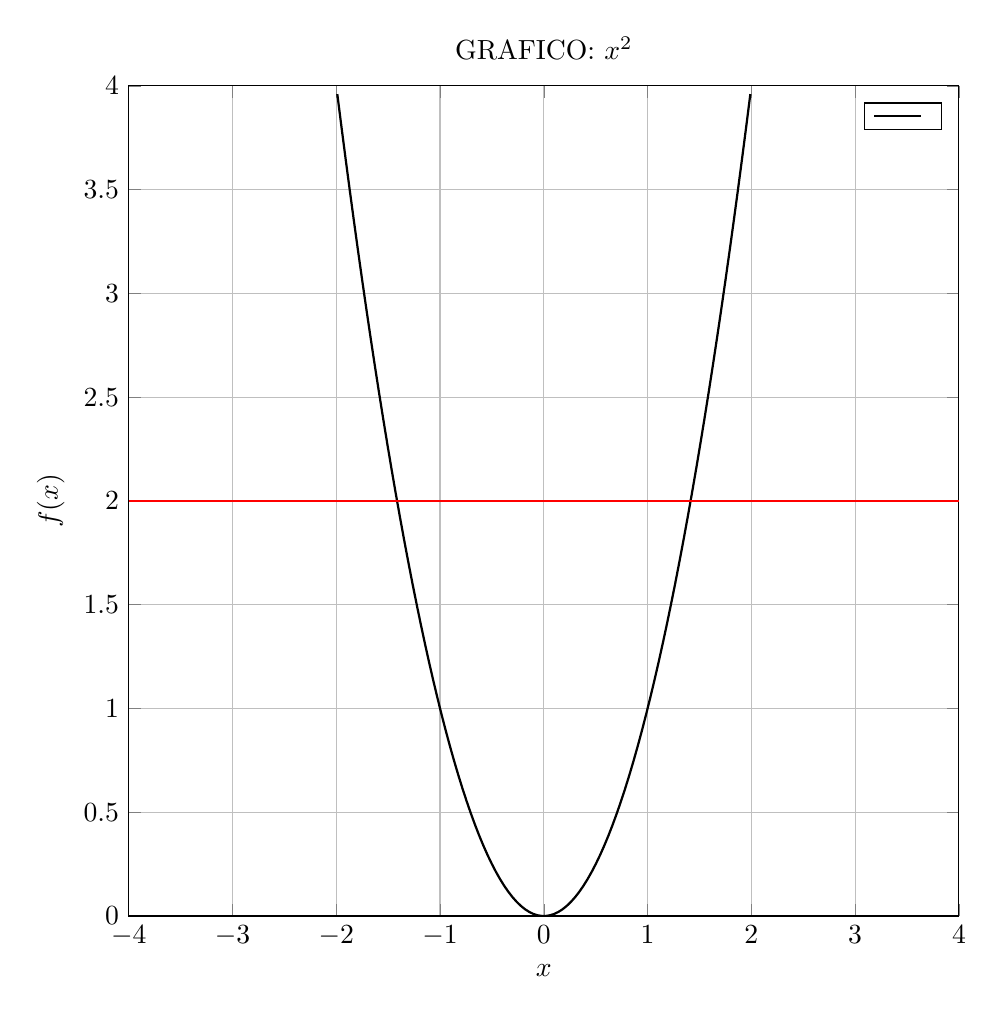
\begin{tikzpicture}
			\begin{axis}[
					title=GRAFICO: $x^{2}$,
					xmin=-4, xmax=4,
					ymin=0,ymax=4,
					restrict y to domain = 0:4, domain=-4:4, width=\textwidth, height=\textwidth, grid=major, samples=200,  ylabel=$f(x)$, xlabel=$x$, legend entries={$ $}]
				\addplot[black, thick] {x^2};
				\addplot[red, thick] {2};
			\end{axis}
		\end{tikzpicture}
	\end{center}
	\begin{itemize}
		\item Non è iniettiva
		\item Non è surgettiva
	\end{itemize}

\end{minipage}
%
\begin{minipage}[t]{0.48\textwidth}
	Esempio 2 $f : \R \rightarrow [0,\infty)$
	\begin{center}
		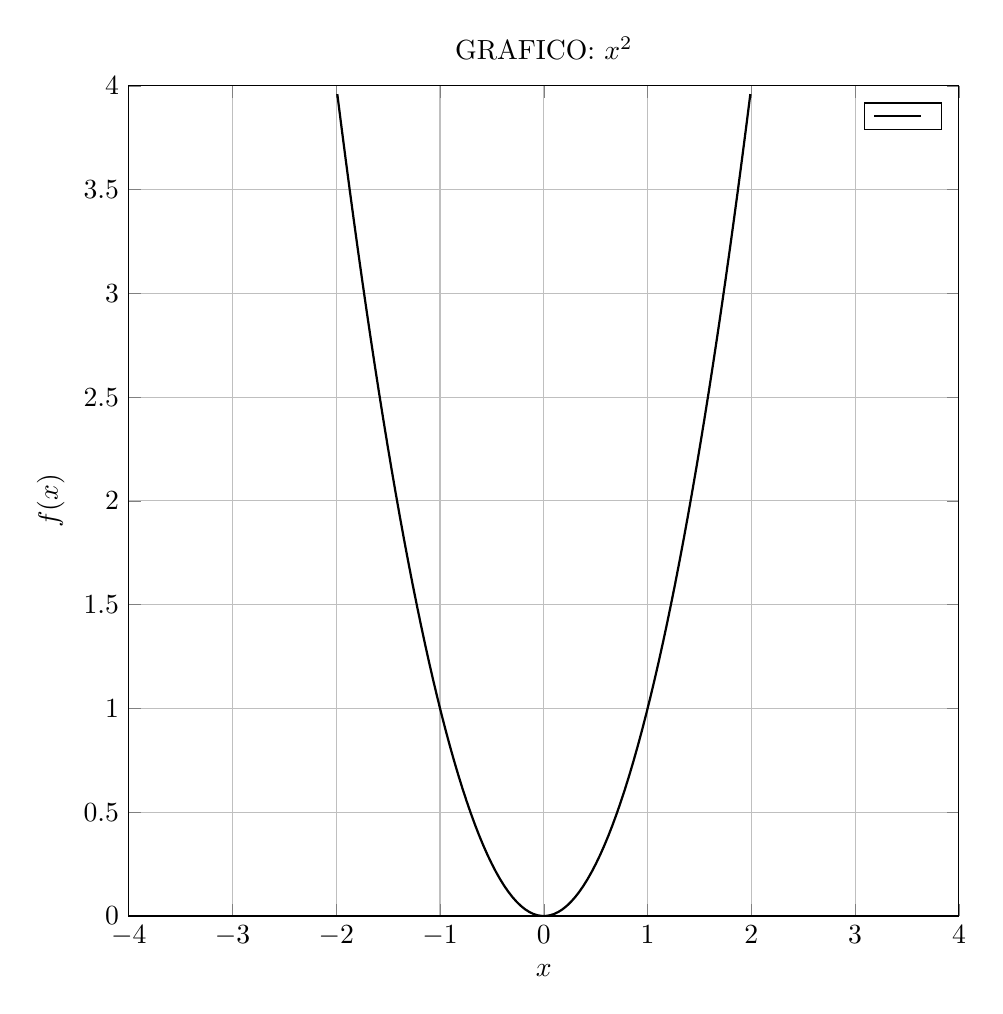
\begin{tikzpicture}
			\begin{axis}[
					title=GRAFICO: $x^2$,
					xmin=-4, xmax=4,
					ymin=0,ymax=4,
					restrict y to domain = 0:4, domain=-4:4, width=\textwidth, height=\textwidth, grid=major, samples=200,  ylabel=$f(x)$, xlabel=$x$, legend entries={$ $}]
				\addplot[black, thick] {x^2};
			\end{axis}
		\end{tikzpicture}
	\end{center}
	\begin{itemize}
		\item Non è iniettiva
		\item E' suriettiva
	\end{itemize}

\end{minipage}
\vskip1cm
\begin{minipage}[t]{0.48\textwidth}
	Esempio 3: $f : [0, \infty) \rightarrow \R$
	\begin{center}
		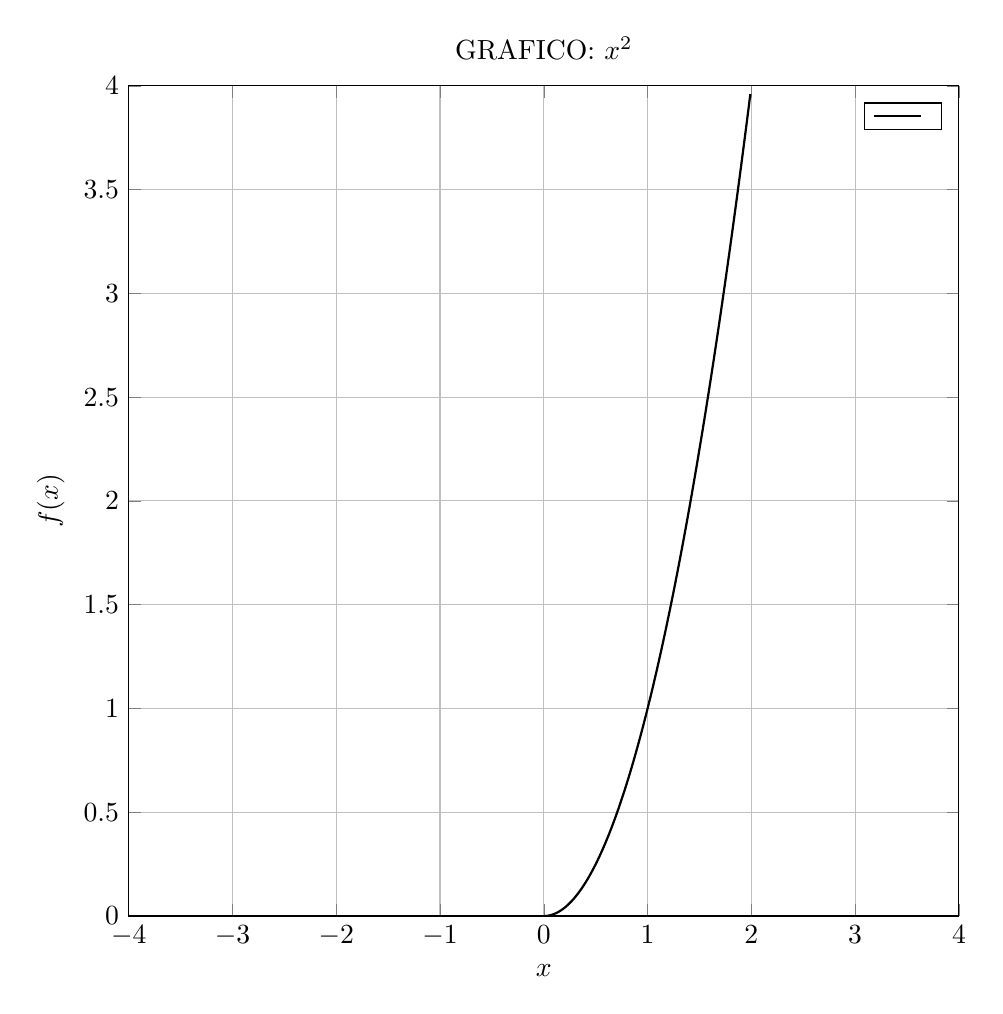
\begin{tikzpicture}
			\begin{axis}[
					title=GRAFICO: $x^2$,
					xmin=-4, xmax=4,
					ymin=0,ymax=4,
					restrict y to domain = 0:4, domain=0:4, width=\textwidth, height=\textwidth, grid=major, samples=200,  ylabel=$f(x)$, xlabel=$x$, legend entries={$ $}]
				\addplot[black, thick] {x^2};
			\end{axis}
		\end{tikzpicture}
	\end{center}
	\begin{itemize}
		\item E' iniettiva
		\item Non è surgettiva
	\end{itemize}

\end{minipage}
%
\begin{minipage}[t]{0.48\textwidth}
	Esempio 3: $f : [0, \infty) \rightarrow [0,\infty)$
	\begin{center}
		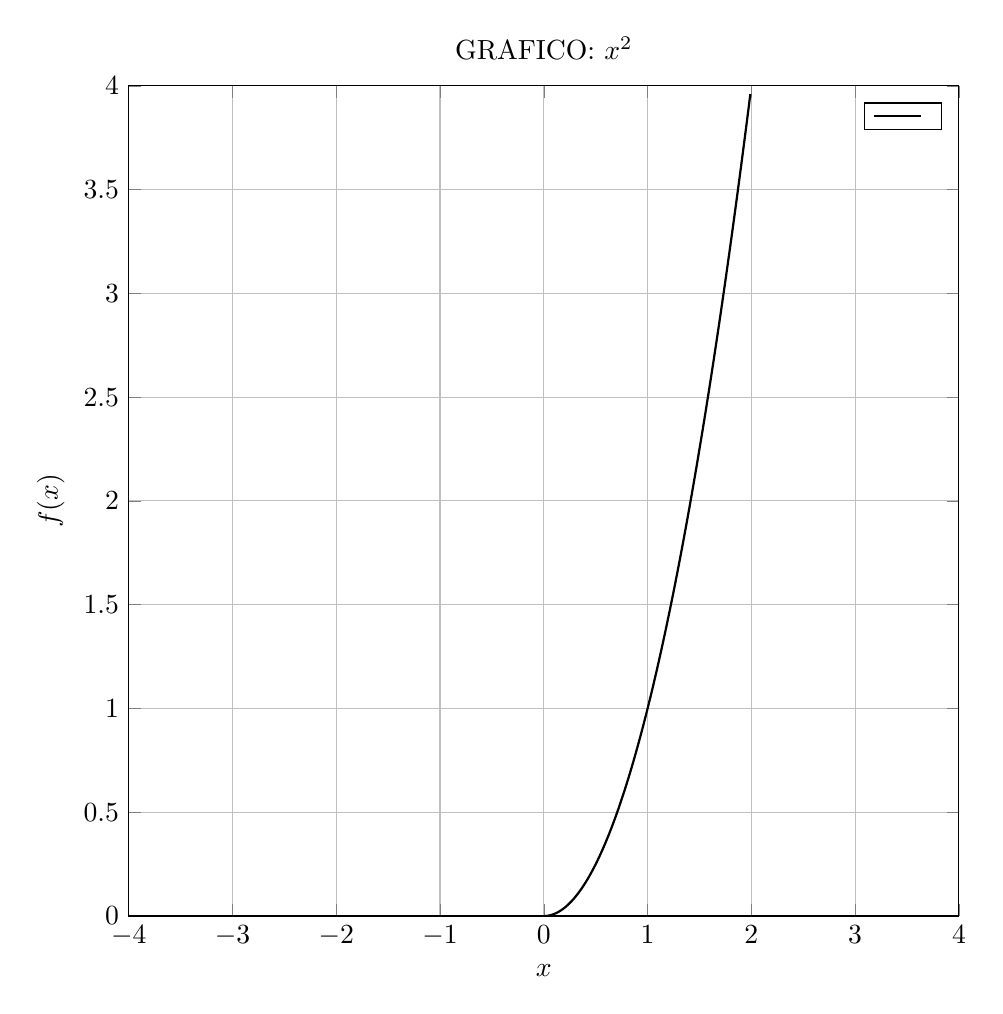
\begin{tikzpicture}
			\begin{axis}[
					title=GRAFICO: $x^2$,
					xmin=-4, xmax=4,
					ymin=0,ymax=4,
					restrict y to domain = 0:4, domain=0:4, width=\textwidth, height=\textwidth, grid=major, samples=200,  ylabel=$f(x)$, xlabel=$x$, legend entries={$ $}]
				\addplot[black, thick] {x^2};
			\end{axis}
		\end{tikzpicture}
	\end{center}
	\begin{itemize}
		\item E' iniettiva
		\item E' surgettiva
	\end{itemize}

\end{minipage}
\subsection{Operazioni sui grafici}
\begin{itemize}
	\item $ f\left( x \right) \to f\left( x \right) +x$ \quad traslazione in verticale (se c è positivo verso l'alto)
	\item $ f\left( x \right) \rightarrow f\left( x+c \right) $ \quad traslazione in orizzontale (se c è positivo verso sinistra)
	\item $f\left( x \right)  \rightarrow -f\left( x \right) $ \quad diventa speculare rispetto ad asse x
	\item $f\left( x \right) \rightarrow f\left( -x \right) $ diventa speculare rispetto all'asse y
	\item $f\left( x \right) \rightarrow \left|f\left( x \right) \right|$ \quad ogni parte negativa diventa ribaltata verso l'alto
	\item $f\left( x \right) \rightarrow f\left( \left|x\right| \right) $ \quad la parte del grafico con $x\ge 0 $ viene riflessa rispetto all'asse y
\end{itemize}
\begin{minipage}[t]{0.48\textwidth}
	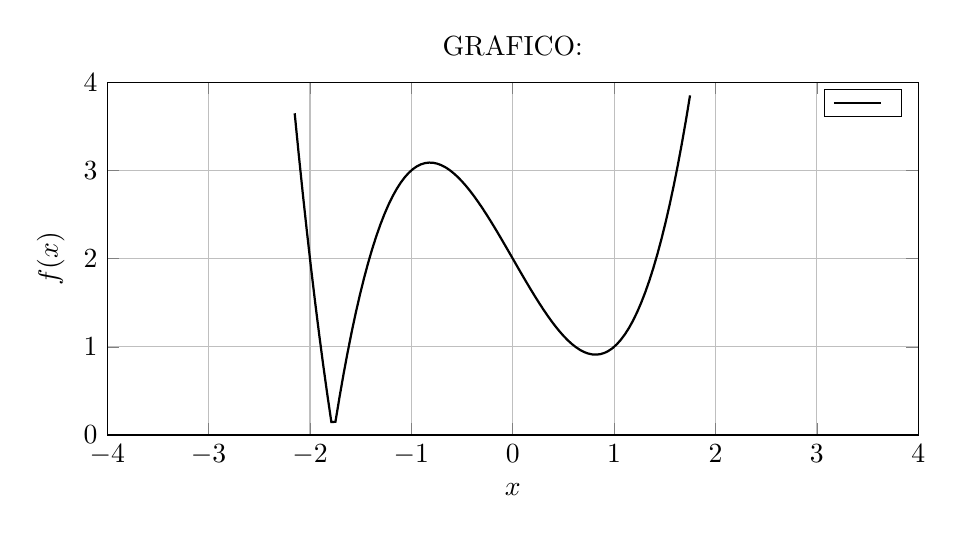
\begin{tikzpicture}
		\begin{axis}[title=GRAFICO: ,
				xmin=-4, xmax=4,
				ymin=0,ymax=4,
				restrict y to domain = 0:4, domain=-4:4, width=0.98\textwidth, height=0.5\textwidth, grid=major, samples=200,  ylabel=$f(x)$, xlabel=$x$, legend entries={$ $}]
			\addplot[black, thick] {abs(x^3-2*x+2)};
		\end{axis}
	\end{tikzpicture}
\end{minipage}
%
\begin{minipage}[t]{0.48\textwidth}

\end{minipage}

\subsection{Risoluzione di equazioni per via grafica}
Esempio 1: \[
	\left|\left|x\right|-1\right|=\frac{1}{2}
\]
\begin{minipage}[t]{0.48\textwidth}
	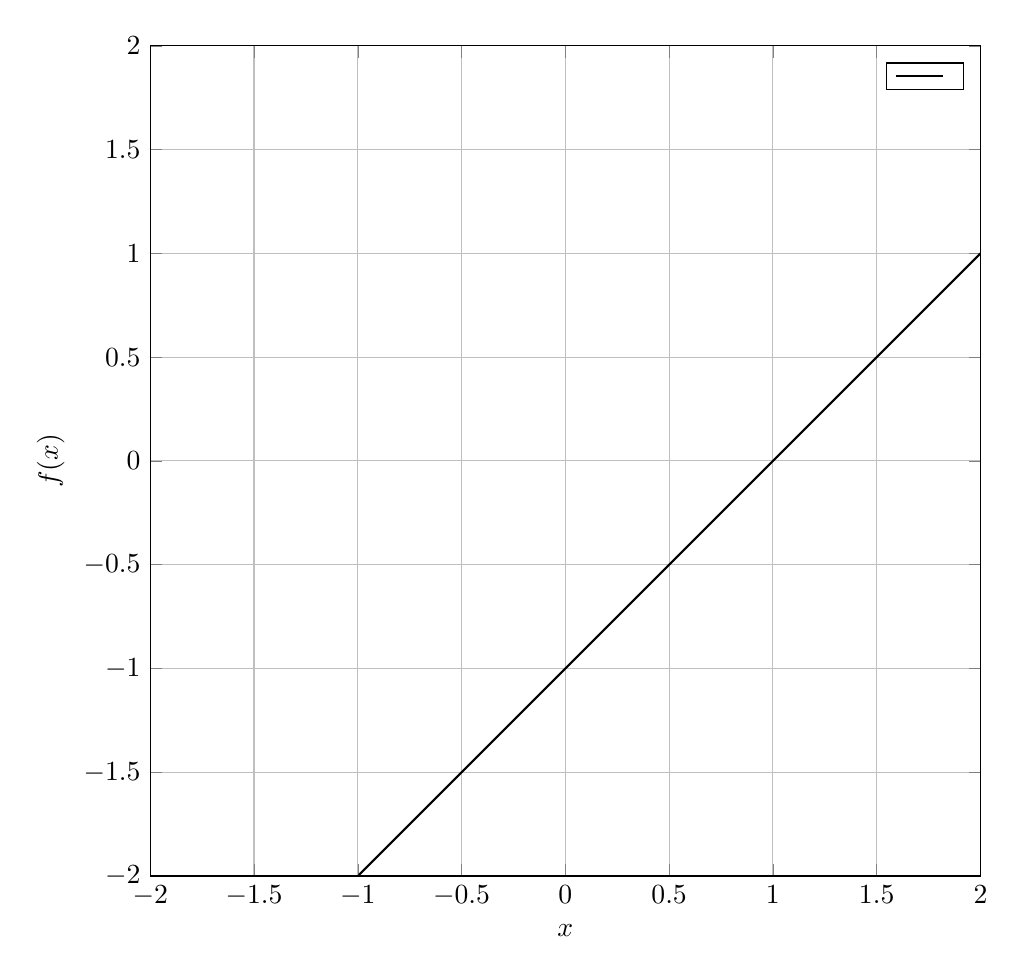
\begin{tikzpicture}
		\begin{axis}[
				xmin=-2, xmax=2,
				ymin=-2,ymax=2,
				restrict y to domain = -2:2, domain=-2:2, width=\textwidth, height=\textwidth, grid=major, samples=200,  ylabel=$f(x)$, xlabel=$x$, legend entries={$ $}]
			\addplot[black, thick] {x-1};
		\end{axis}
	\end{tikzpicture}
\end{minipage}
%
\begin{minipage}[t]{0.48\textwidth}
	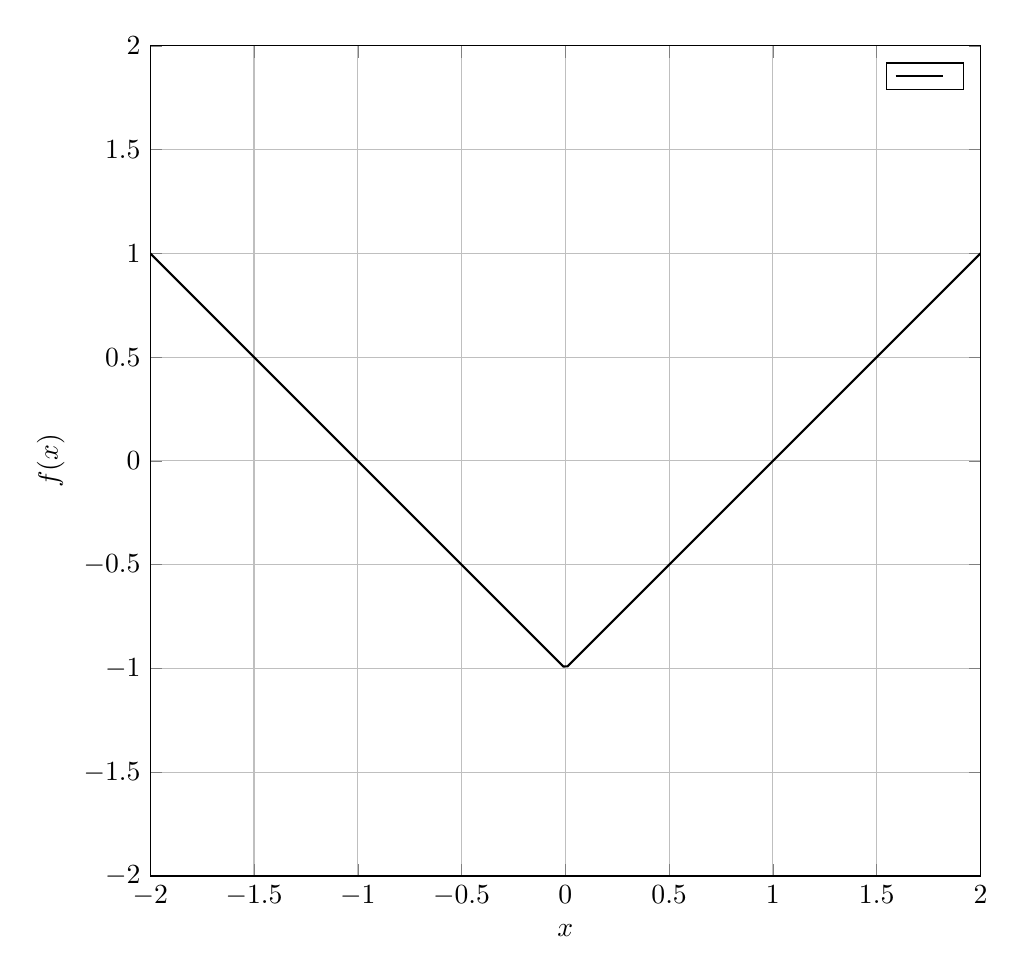
\begin{tikzpicture}
		\begin{axis}[
				xmin=-2, xmax=2,
				ymin=-2,ymax=2,
				restrict y to domain = -2:2, domain=-2:2, width=\textwidth, height=\textwidth, grid=major, samples=200,  ylabel=$f(x)$, xlabel=$x$, legend entries={$ $}]
			\addplot[black, thick] {abs(x)-1};
		\end{axis}
	\end{tikzpicture}
\end{minipage}
\begin{center}
	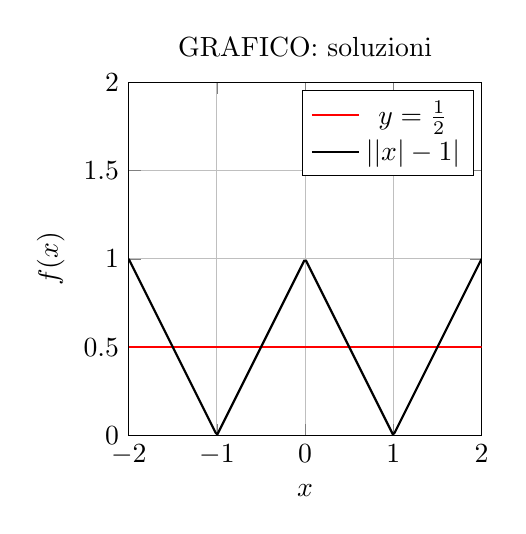
\begin{tikzpicture}
		\begin{axis}[
				title=GRAFICO: soluzioni ,
				xmin=-2, xmax=2,
				ymin=0,ymax=2,
				restrict y to domain = -2:2, domain=-2:2, width=0.5\textwidth, height=0.5\textwidth, grid=major, samples=200,  ylabel=$f(x)$, xlabel=$x$, legend entries={$y=\frac{1}{2}$, $ \left|\left|x\right|-1\right|$}]
			\addplot[red, thick] {0.5};
			\addplot[black, thick] {abs(abs(x)-1)};
		\end{axis}
	\end{tikzpicture}
\end{center}
Esercizio: determinare al variare di
$\lambda  \in  \R$ quali sono le soluzioni dell'equazione \[
	\left|\left( x+3 \right) ^3 -2\right|=\lambda
\]
\section{Potenze, esponenziali, funzioni trigonometriche}
\subsection{Potenze pari}


\begin{minipage}[t]{0.48\textwidth}
	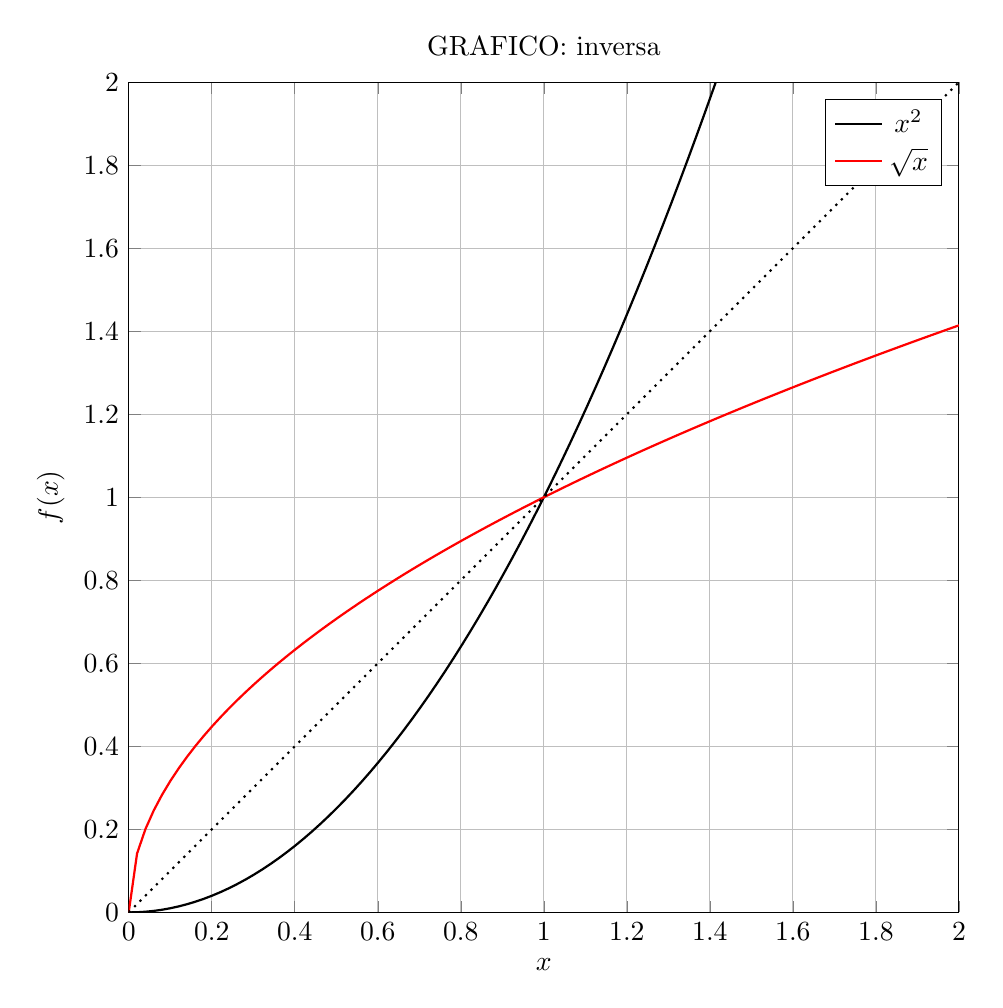
\begin{tikzpicture}
		\begin{axis}[
				title=GRAFICO: inversa,
				xmin=0, xmax=2,
				ymin=0,ymax=2,
				restrict y to domain = 0:4, domain=0:4, width=\textwidth, height=\textwidth, grid=major, samples=200,  ylabel=$f(x)$, xlabel=$x$, legend entries={$ x^2$, $\sqrt{x} $}]
			\addplot[black, thick] {x^2};
			\addplot[red, thick] {sqrt(x)};
			\addplot[dotted, thick] {x};
		\end{axis}
	\end{tikzpicture}
\end{minipage}
%
\begin{minipage}[t]{0.48\textwidth}
	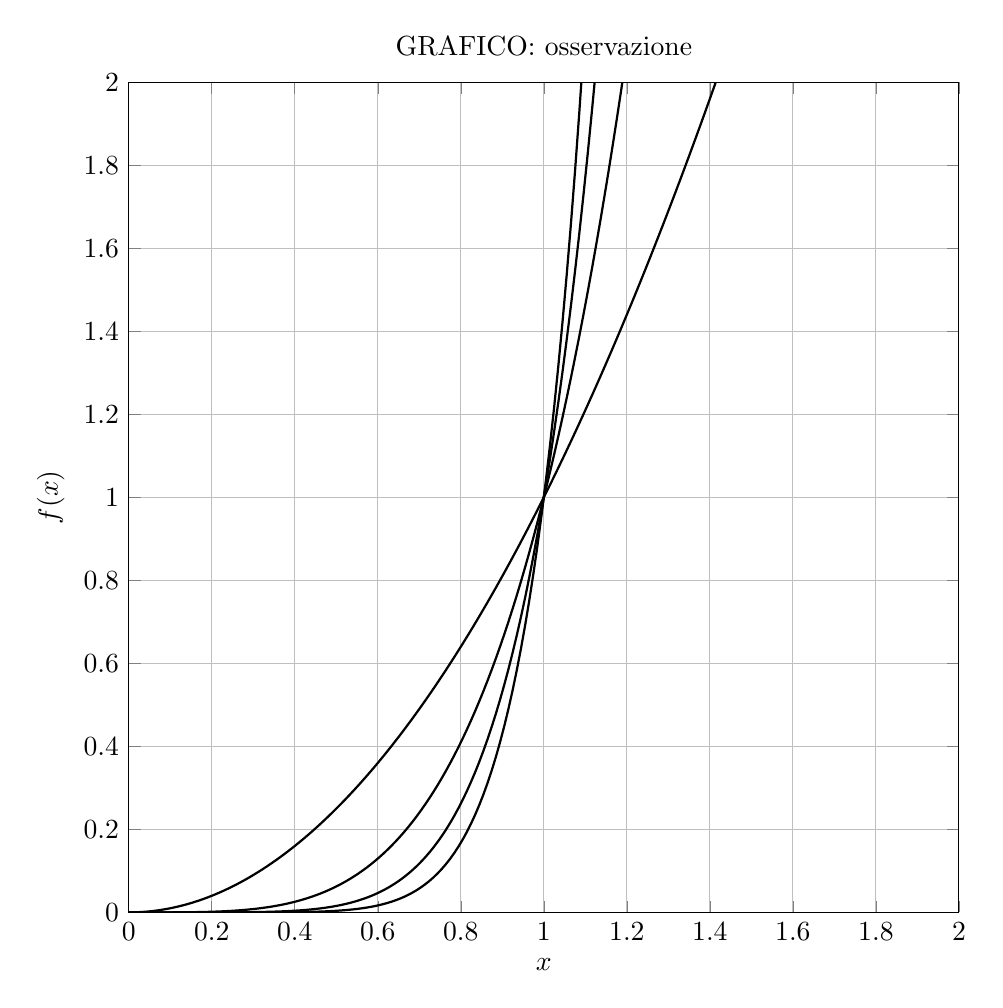
\begin{tikzpicture}
		\begin{axis}[
				title=GRAFICO: osservazione,
				xmin=0, xmax=2,
				ymin=0,ymax=2,
				restrict y to domain = 0:3, domain=0:2, width=\textwidth, height=\textwidth, grid=major, samples=200,  ylabel=$f(x)$, xlabel=$x$]
			\addplot[black, thick] {x^2};
			\addplot[black, thick] {x^4};
			\addplot[black, thick] {x^6};
			\addplot[black, thick] {x^8};
		\end{axis}
	\end{tikzpicture}
\end{minipage}

\subsection{Potenze dispari}
\begin{center}
	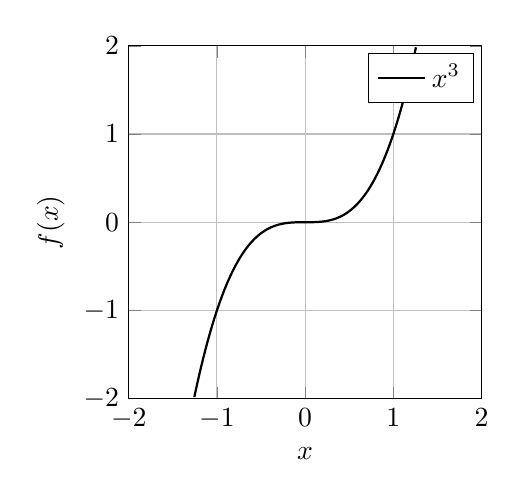
\begin{tikzpicture}
		\begin{axis}[
				xmin=-2, xmax=2,
				ymin=-2,ymax=2,
				restrict y to domain = -2:2, domain=-2:2, width=0.5\textwidth, height=0.5\textwidth, grid=major, samples=200,  ylabel=$f(x)$, xlabel=$x$, legend entries={$ x^3 $}]
			\addplot[black, thick] {x^3};
		\end{axis}
	\end{tikzpicture}
\end{center}

\textbox{OSS: se una funzione $f\left( x \right) $ è iniettiva e $a = b$ allora $f\left( a \right) = f\left( b \right) $. Se $ a > b$ allora $f\left( x \right) > f\left( b \right) $ se $f$ è crescente}
\subsection{Esponenziale e logaritmo}
\begin{minipage}[t]{0.48\textwidth}
	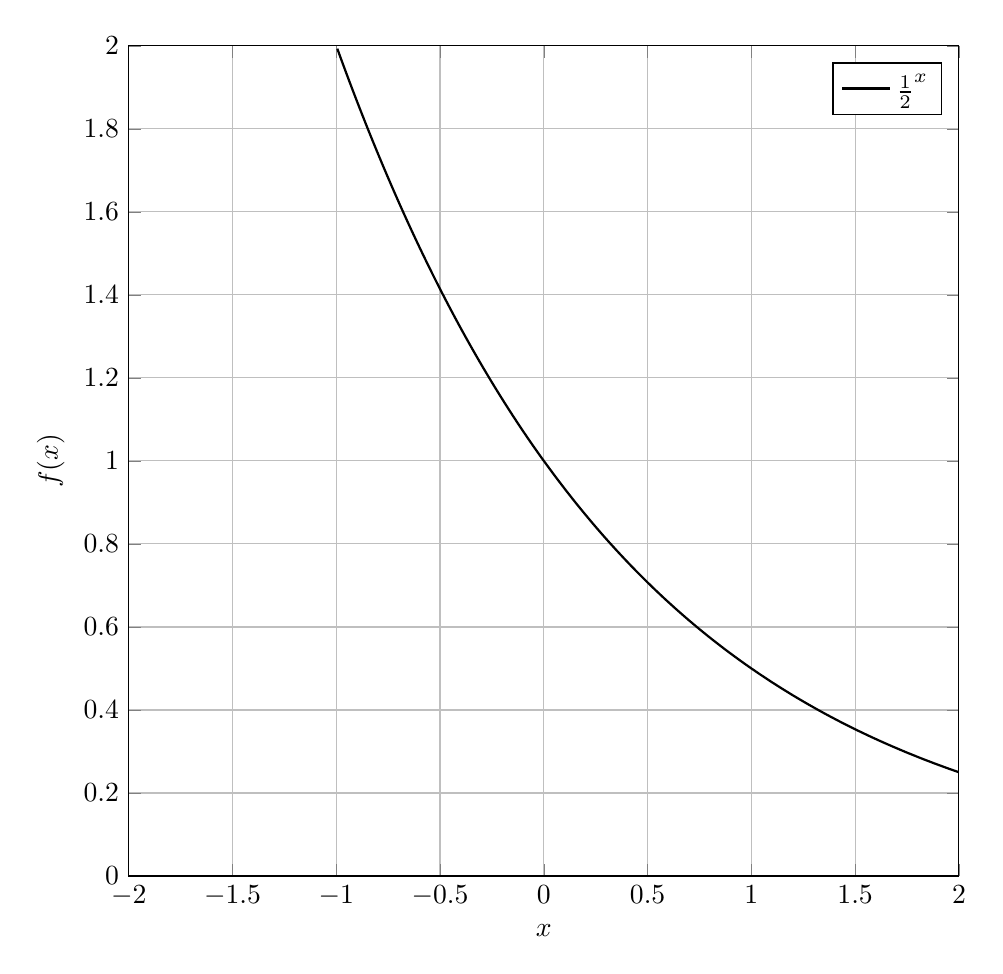
\begin{tikzpicture}
		\begin{axis}[
				xmin=-2, xmax=2,
				ymin=0,ymax=2,
				restrict y to domain = -2:2, domain=-2:2, width=\textwidth, height=\textwidth, grid=major, samples=200,  ylabel=$f(x)$, xlabel=$x$, legend entries={$\frac{1}{2}^{x}$}]
			\addplot[black, thick] {0.5^x};
		\end{axis}
	\end{tikzpicture}
\end{minipage}
%
\begin{minipage}[t]{0.48\textwidth}
	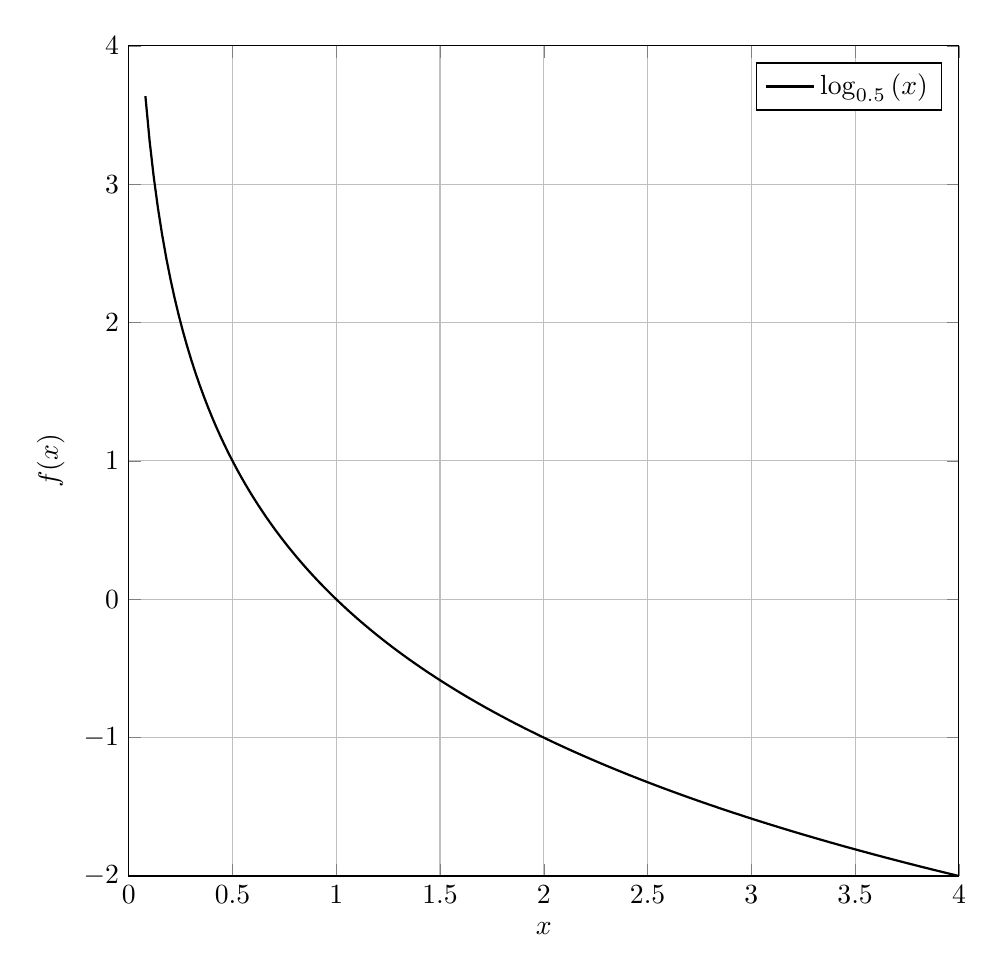
\begin{tikzpicture}
		\begin{axis}[
				xmin=0, xmax=4,
				ymin=-2,ymax=4,
				restrict y to domain = -2:4, domain=0:4, width=\textwidth, height=\textwidth, grid=major, samples=200,  ylabel=$f(x)$, xlabel=$x$, legend entries={$ \log_{0.5} \left( x \right) $}]
			\addplot[black, thick] {ln(x)/ln(0.5)};
		\end{axis}
	\end{tikzpicture}
\end{minipage}
\[
	e^{x} + e^{y} = e^{x+y} \quad \left( e^{x} \right) ^{y}= e^{xy}
\]

\subsection{Funzioni trigonometriche}
\begin{minipage}[t]{0.48\textwidth}
	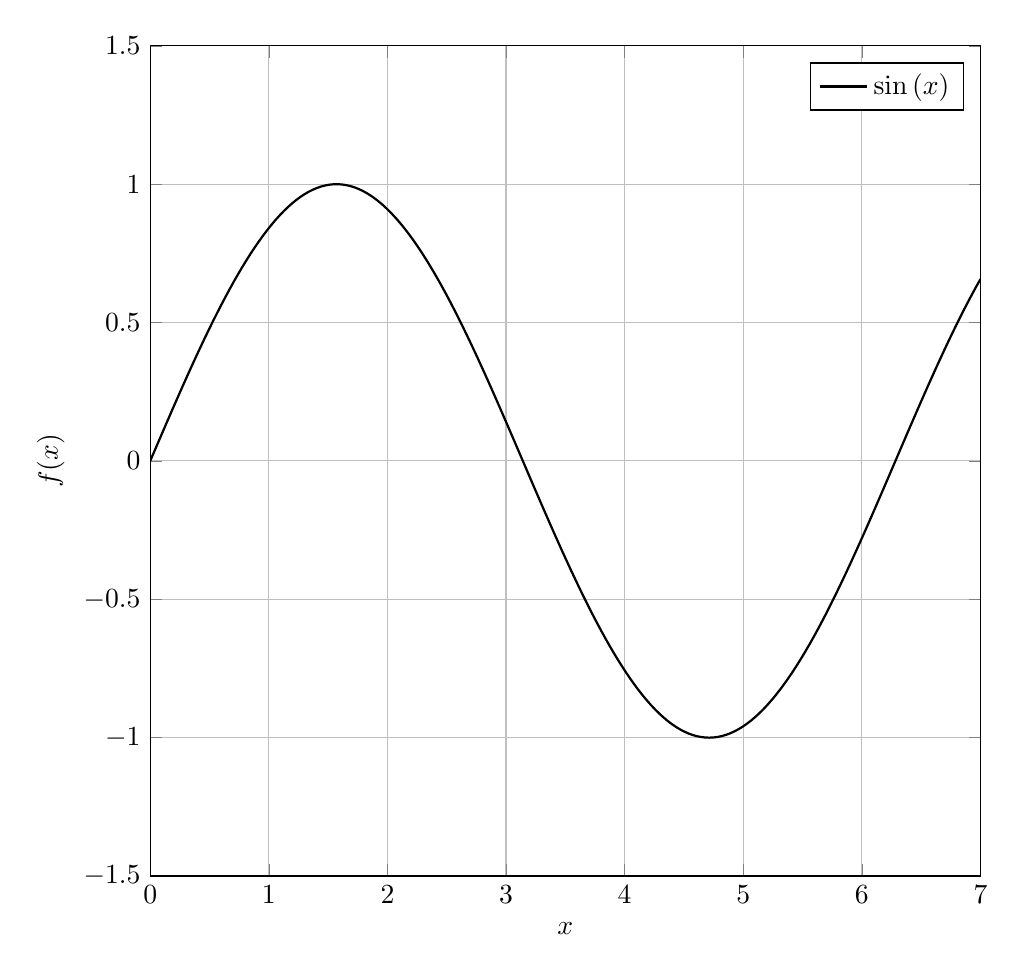
\begin{tikzpicture}
		\begin{axis}[
				xmin=0, xmax=7,
				ymin=-1.5,ymax=1.5,
				restrict y to domain =-2:2, domain=0:7, width=\textwidth, height=\textwidth, grid=major, samples=200,  ylabel=$f(x)$, xlabel=$x$, legend entries={$ \sin\left( x \right)  $}]
			\addplot[black, thick] {sin(deg(x))};
		\end{axis}
	\end{tikzpicture}
\end{minipage}
%
\begin{minipage}[t]{0.48\textwidth}
	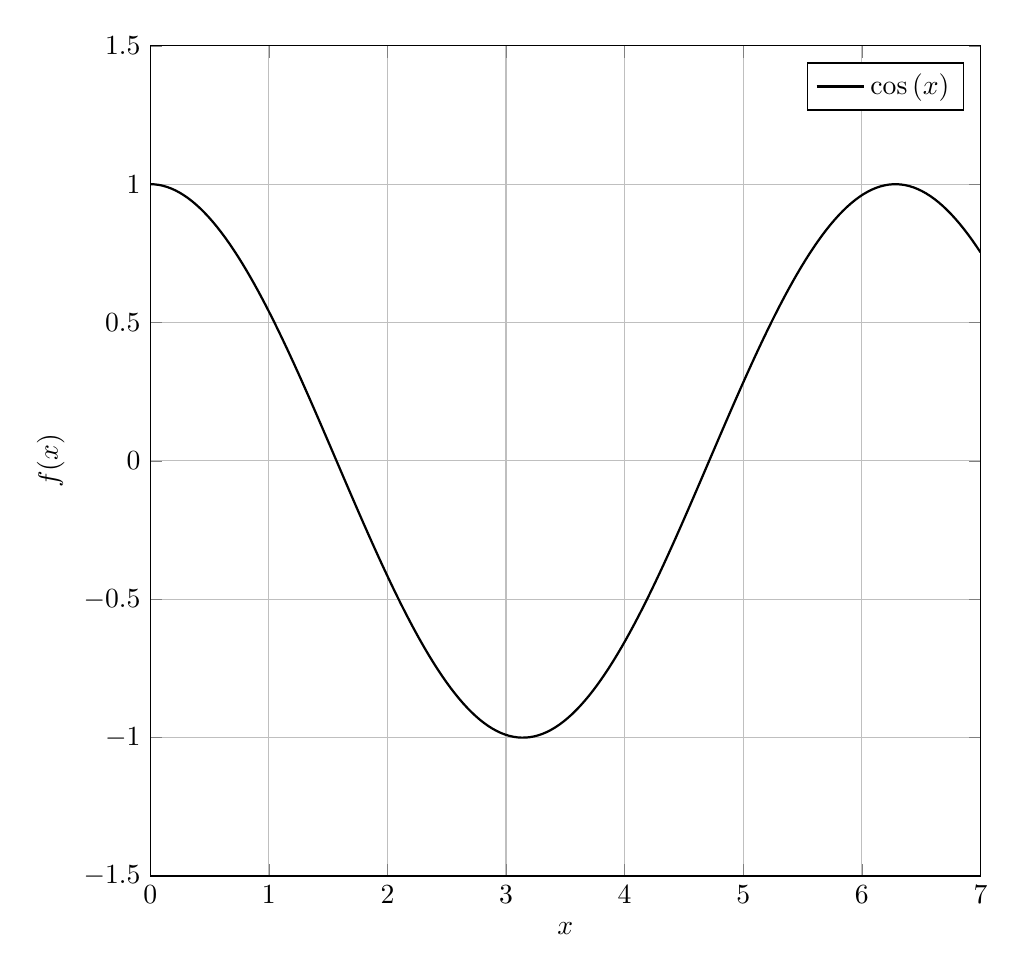
\begin{tikzpicture}
		\begin{axis}[
				xmin=0, xmax=7,
				ymin=-1.5,ymax=1.5,
				restrict y to domain =-2:2, domain=0:7, width=\textwidth, height=\textwidth, grid=major, samples=200,  ylabel=$f(x)$, xlabel=$x$, legend entries={$ \cos\left( x \right)  $}]
			\addplot[black, thick] {cos(deg(x))};
		\end{axis}
	\end{tikzpicture}
\end{minipage}

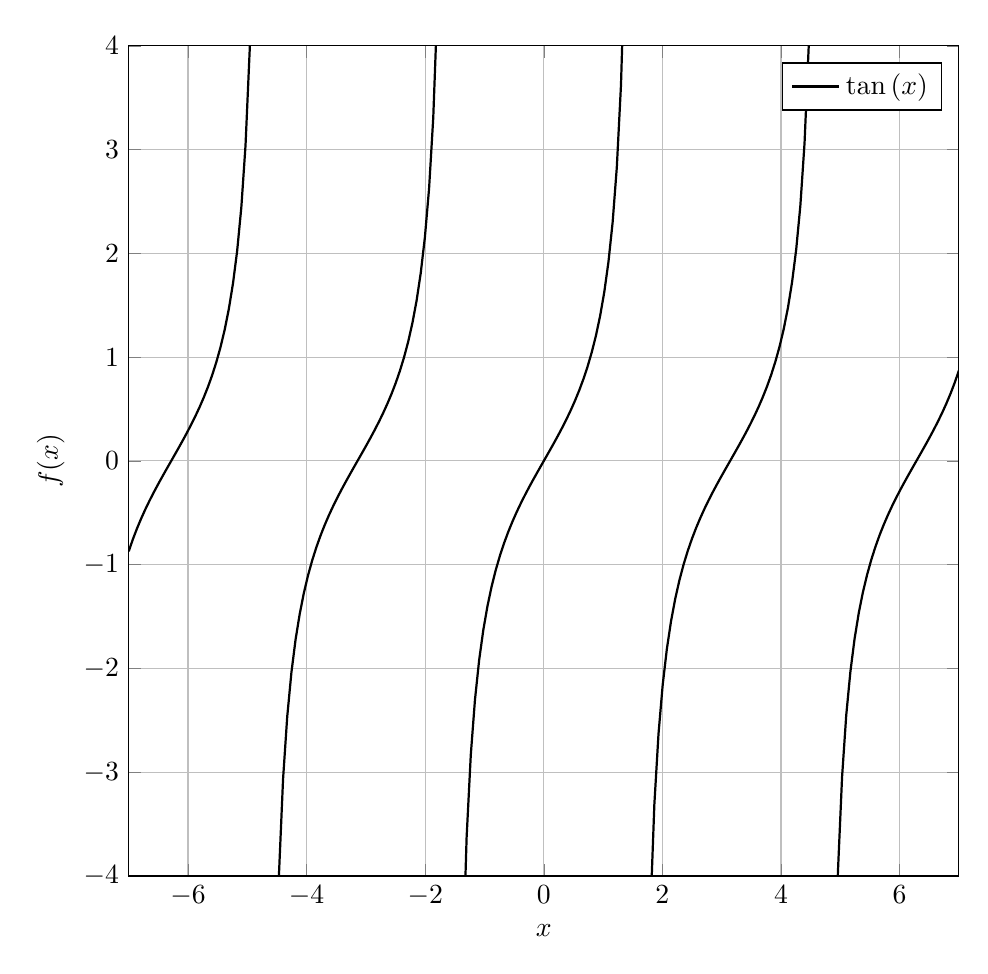
\begin{tikzpicture}
	\begin{axis}[
			xmin=-7, xmax=7,
			ymin=-4,ymax=4,
			restrict y to domain =-7:7, domain=-7:7, width=\textwidth, height=\textwidth, grid=major, samples=200,  ylabel=$f(x)$, xlabel=$x$, legend entries={$ \tan \left( x \right) $}]
		\addplot[black, thick] {tan(deg(x))};
	\end{axis}
\end{tikzpicture}
\subsubsection{Inverto il seno}
Il seno non è ne iniettivo ne surgettivo a meno che non lo consideri come:
\[
	f: \left[ -\frac{\pi}{2}, \frac{\pi}{2} \right] \rightarrow \left[ -1,1 \right]
\]
Il coseno non è ne iniettivo ne survettivo a meno che non lo si consideri come:
\[
	f: \left[ 0, \pi \right] \rightarrow \left[ -1,1 \right]
\]


\begin{minipage}[t]{0.48\textwidth}
	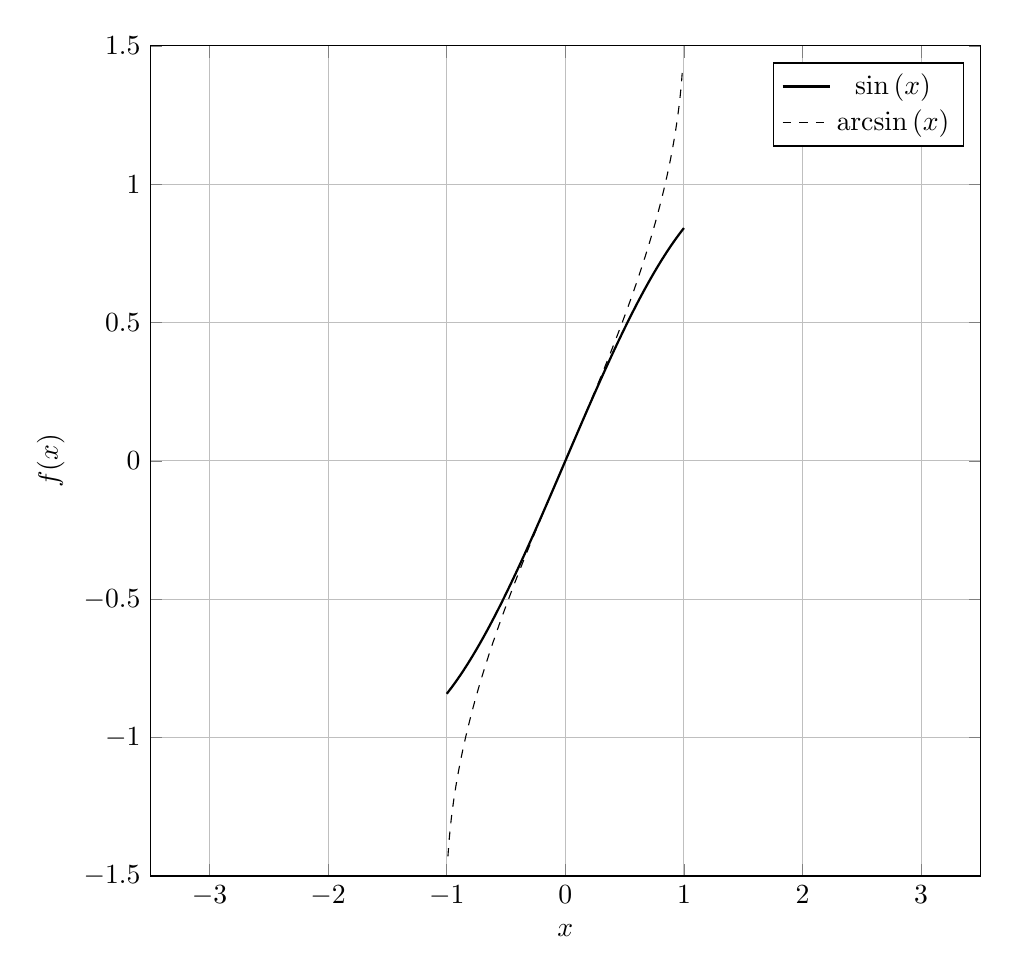
\begin{tikzpicture}
		\begin{axis}[
				xmin=-3.5, xmax=3.5,
				ymin=-1.5,ymax=1.5,
				restrict y to domain = -1.5:1.5, domain=-1:1, width=\textwidth, height=\textwidth, grid=major, samples=200,  ylabel=$f(x)$, xlabel=$x$, legend entries={$ \sin\left( x \right)  $, $ \arcsin \left( x \right)  $}]
			\addplot[black, thick] {sin(deg(x))};
			\addplot[dashed, domain=-1:1] {asin(x)/180*pi};
		\end{axis}
	\end{tikzpicture}
\end{minipage}
%
\begin{minipage}[t]{0.48\textwidth}
	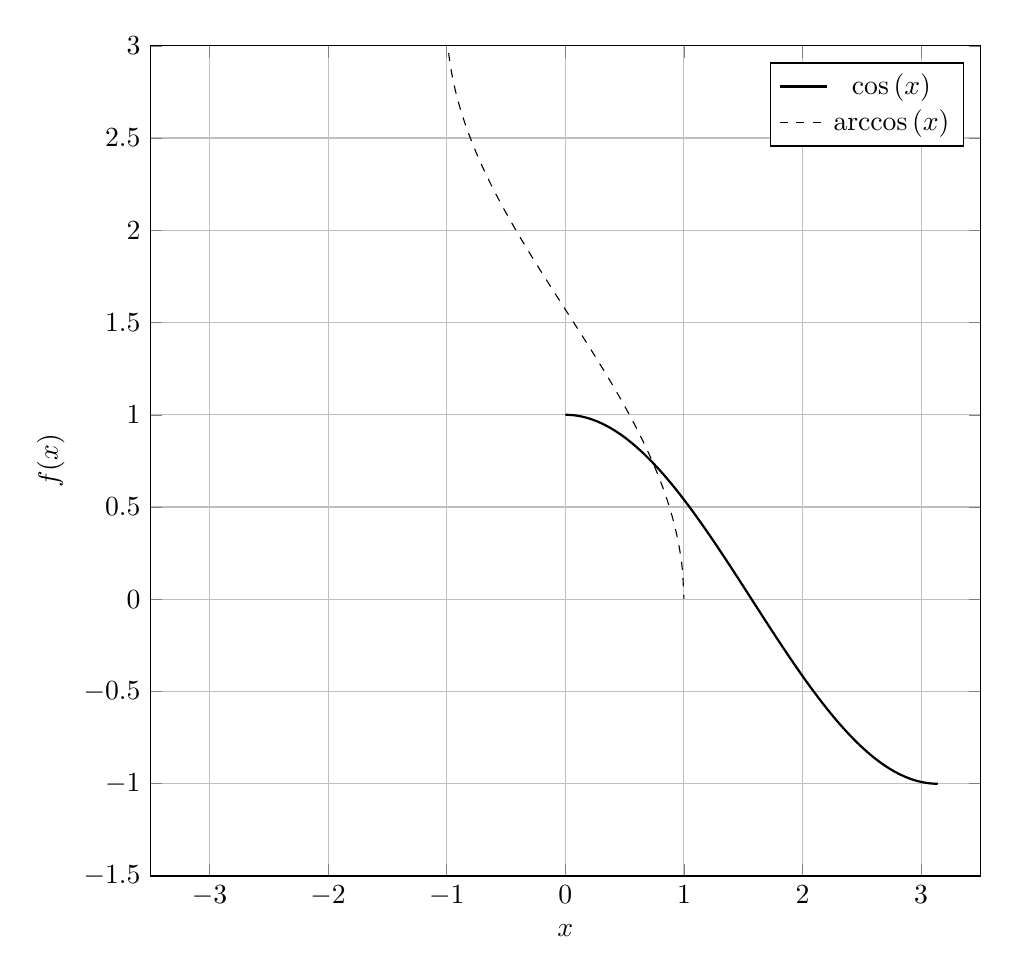
\begin{tikzpicture}
		\begin{axis}[
				xmin=-3.5, xmax=3.5,
				ymin=-1.5,ymax=3,
				restrict y to domain = -10:10, domain=0:3.14, width=\textwidth, height=\textwidth, grid=major, samples=200,  ylabel=$f(x)$, xlabel=$x$, legend entries={$ \cos \left( x \right) 	 $, $ \arccos \left( x \right) $}]
			\addplot[black, thick] {cos(deg(x))};
			\addplot[dashed, domain=-1:1] {acos(x)/180*pi};
		\end{axis}
	\end{tikzpicture}

\end{minipage}
\subsection{Funzioni iperboliche}
\[
	\cosh = \frac{e^{x} + e^{-x}}{2} \rightarrow pari
\]
\[
	\sinh = \frac{e^{x} - e^{-x}}{2} \rightarrow dispari
\]
\[
	\tanh = \frac{\sinh}{\cosh} \rightarrow dispari
\]
\begin{minipage}[t]{0.48\textwidth}
	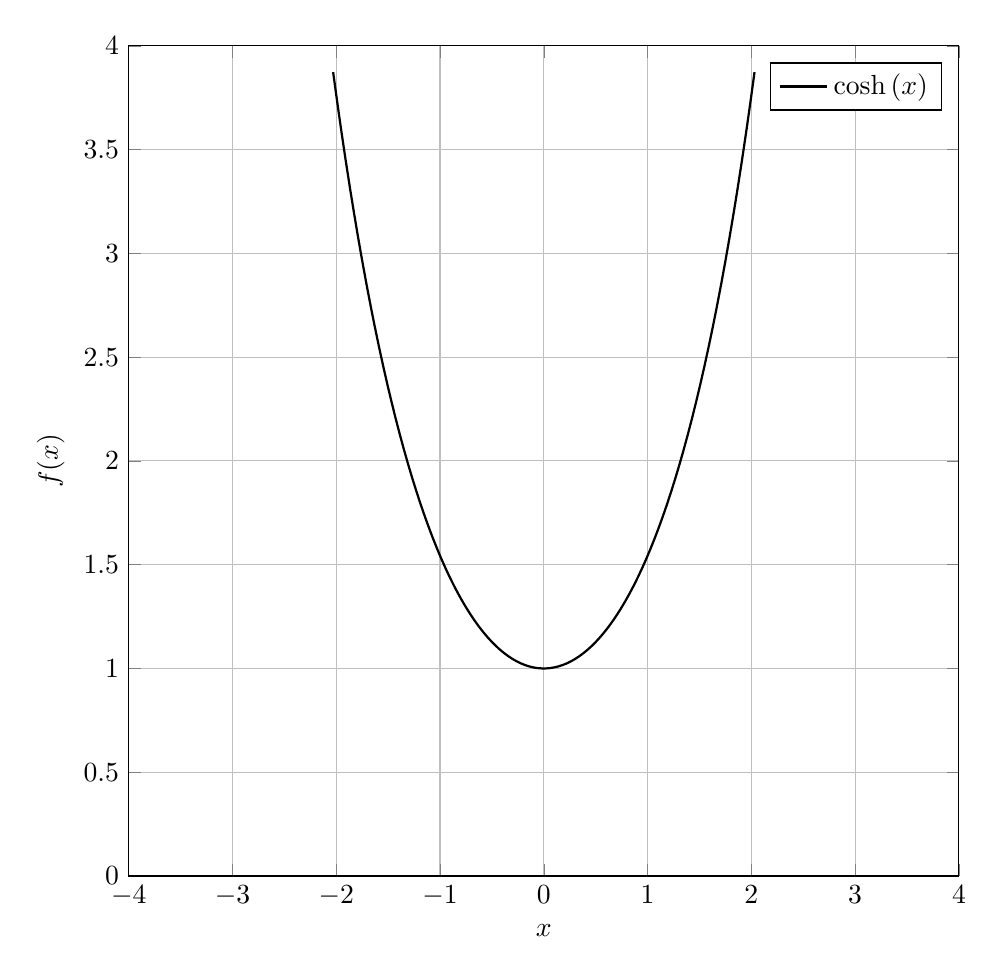
\begin{tikzpicture}
		\begin{axis}[
				xmin=-4, xmax=4,
				ymin=0,ymax=4,
				restrict y to domain = 0:4, domain=-4:4, width=\textwidth, height=\textwidth, grid=major, samples=200,  ylabel=$f(x)$, xlabel=$x$, legend entries={$ \cosh \left( x \right) $}]
			\addplot[black, thick] {cosh(x)};
		\end{axis}
	\end{tikzpicture}
\end{minipage}
%
\begin{minipage}[t]{0.48\textwidth}
	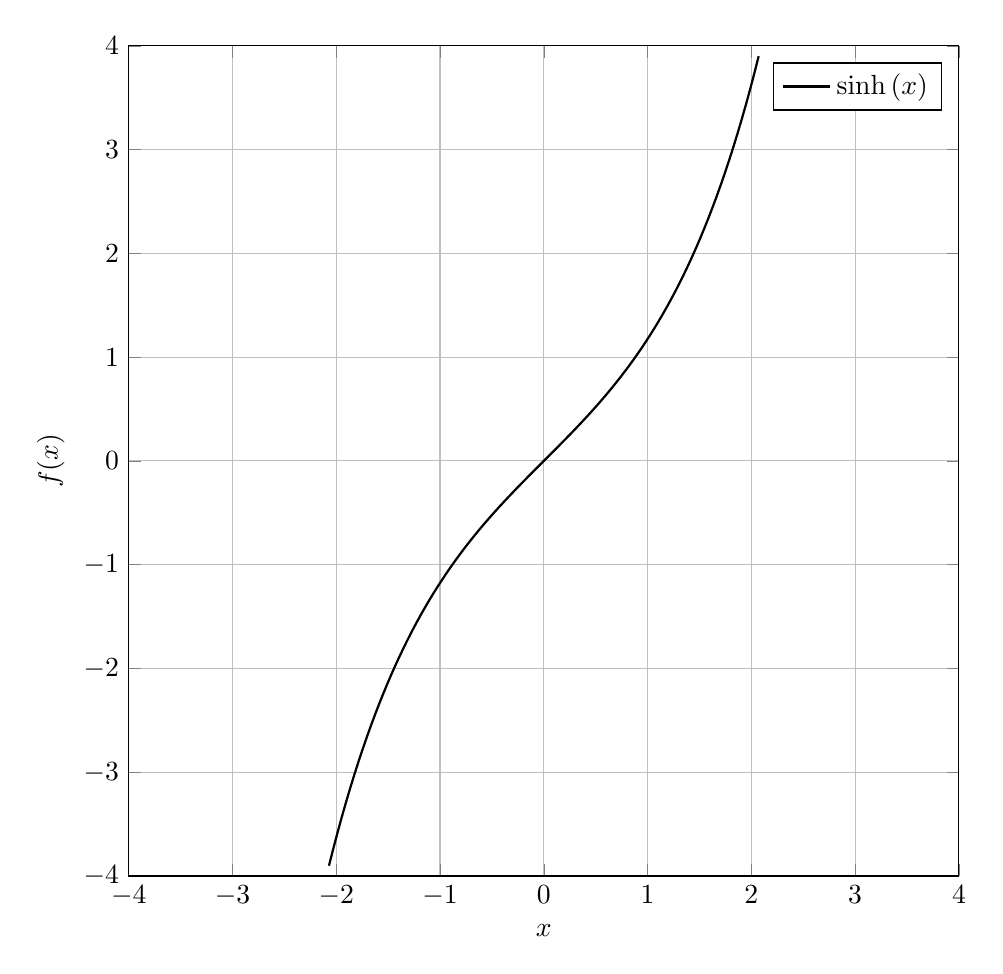
\begin{tikzpicture}
		\begin{axis}[
				xmin=-4, xmax=4,
				ymin=-4,ymax=4,
				restrict y to domain = -4:4, domain=-4:4, width=\textwidth, height=\textwidth, grid=major, samples=200,  ylabel=$f(x)$, xlabel=$x$, legend entries={$ \sinh \left( x \right) $}]
			\addplot[black, thick] {sinh(x)};
		\end{axis}
	\end{tikzpicture}
\end{minipage}

\begin{center}
	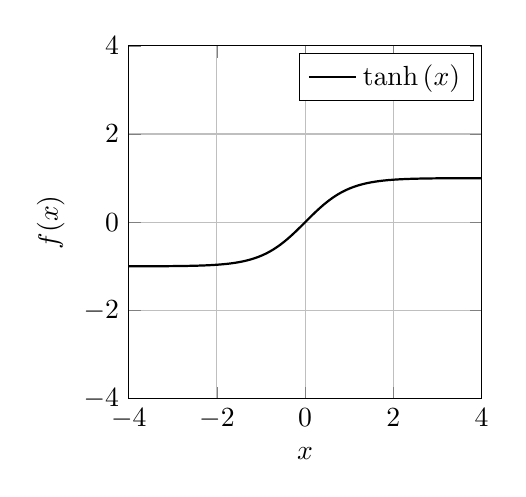
\begin{tikzpicture}
		\begin{axis}[
				xmin=-4, xmax=4,
				ymin=-4,ymax=4,
				restrict y to domain = -4:4, domain=-4:4, width=0.5\textwidth, height=0.5\textwidth, grid=major, samples=200,  ylabel=$f(x)$, xlabel=$x$, legend entries={$ \tanh \left( x \right)  $}]
			\addplot[black, thick] {tanh(x)};
		\end{axis}
	\end{tikzpicture}
\end{center}


\subsection{Formule trigonometria iperbolica}
\textbox{Queste formule sono molto simili alle formule della trigonometria tradizionale}
\[
	\sin\left( 2x \right) = 2 \sin \left( x \right) \cos\left( x \right)
\]
\[
	\sinh \left( 2x \right)  = \frac{e^{2x} - e ^{-2x}}{2} = \frac{\left( e^{x} \right) ^{2} - \left( e^{-x} \right) ^{2}}{2}= \frac{\left( e^{x}- e^{-x} \right)  \left( e^{x} + e^{-x} \right)}{2} = 2 \sinh\left( x \right) \cosh \left( x \right)
\]
Formula fondamentale della trigonometria \[
	\sinh ^2 x = \left( \frac{e^{x} - e ^{ -x}}{2} \right) ^2 = \frac{e^{2} + e^{2x}- 2}{4}
\]
\[
	\cosh ^2 x = \left( \frac{e^{x} + e ^{ -x}}{2} \right) ^2 = \frac{e^{2} + e^{2x}+ 2}{4}
\]
\[
	\cosh ^2x - \sinh ^2 x = 1
\]
\section{Esercizi}
\subsection{Esercizio 1}

\teorema{Insiemi limitati}{Se un insieme $S \neq \emptyset$ è \underline{limitato superiormente/inferiormente} esso ammette \underline{estremo superiore/inferiore}}
\label{teo6}
\bigbox{
	Dato un un insieme $S$ limitato inferiormente ma non superiormente e un insieme $L$ costituito da tutti i minoranti di $S$ allora \[
		\text{sup}L \text{ esiste e sup}L= \text{ inf}A
	\]
}
\begin{itemize}
	\item L'insieme $S$ denota tutti i maggioranti di $L$
	      \[
		      y \ge x \quad \forall y  \in S, x  \in L
	      \]
	\item Vito che $L$ ammette maggioranti, esso è limitato superiormente e per il teorema \ref{teo6} ammette estremo superiore sup$L$=$\beta$
	\item Visto che l'insieme $S$ denota i maggioranti di $L$, allora \[
		      \text{ se } x < \beta \rightarrow \text{ x non è maggiorante } \rightarrow x  \not\in S
	      \]
	      al contrario, tuttavia
	      \[
		      \text{ se } x  \in S \rightarrow x \ge \beta \rightarrow \beta\text{ è minorante di } S
	      \]
	\item Se prendo $\epsilon > \beta$ so che questa non appartiene a $L $ in quanto è più grande di un suo maggiorante, dunque \[
		      \text{ se  } \epsilon > \beta \rightarrow \epsilon  \not\in L \rightarrow \text{ non è minorante di S }
	      \]
	\item Dunque $\beta$:
	      \begin{enumerate}
		      \item E minorante di S
		      \item Se $\epsilon > \beta \rightarrow \epsilon \text{ non è minorante di } S$
	      \end{enumerate}
	      \bigbox{ $\beta $ è dunque \underline{estremo inferiore di $S$}\[
			      \text{ supL}= \text{ infS }=\beta
		      \] }
\end{itemize}
\subsection{Esercizio 2}
Dato l'insieme
\[
	A = \left\{ a_n = \frac{\cos \left( \pi n  \right)}{n^2 + 1}, \quad n  \in \N  \right\}
\]
si determini limite superiore, inferiore, massimo e minimo se presenti.
\begin{itemize}
	\item Scrivo qualche termine  \[
		      a_0 = 1 , a_1 = -\frac{1}{2}, a_2= \frac{1}{5}, a_3 = -\frac{1}{10}, a_4=\frac{1}{17}
	      \]
	\item Osservo che \[
		      \left|a_n\right|> \left|a_n+1\right| \quad \forall n  \in  \N
	      \]
	\item $\left|a_n\right| = \left| \frac{\cos \left( \pi n \right) }{n^2 +1}\right|= \frac{1}{n^2 + 1}$ in quanto $\cos\left( \pi n \right) $ è sempre uguale a $\pm 1$
	\item Risolvo disequazione \rarr è vera $ \forall n  \in  \N$
	      \[
		      \frac{1}{n^2 +1} \ge \frac{1}{\left( n+1 \right) ^2 + 1}
	      \]
	\item Visto che la successione decresce in valore assoluto posso affermare che
\end{itemize}

\begin{table}[h!]
	\centering
	\begin{tabular}{|ll|}
		\hline
		Estremo superiore & 1              \\
		Estremo inferiore & $-\frac{1}{2}$ \\
		Massimo           & 1              \\
		Minimo            & $-\frac{1}{2}$ \\
		\hline
	\end{tabular}
\end{table}
\subsection{Esercizio 3}
Dato l'insieme
\[
	A = \left\{ a_n = \frac{N^2 - 5}{n^2 +2}, \quad  n  \in  \N \right\}
\]

si determini limite superiore, inferiore, massimo e minimo se presenti.
\begin{itemize}
	\item Scrivo qualche termine
	      \[
		      a_0 = \frac{5}{2}, a_1 = - \frac{4}{3} , a-2 = -\frac{1}{6}, a_3 =\frac{4}{11}
	      \]
	\item Noto che termini sono crescenti e lo verifico risolvendo la disequazione: \[
		      \frac{\left( n+1 \right) ^2 -5}{\left( n+1 \right) ^2 + 2} > \frac{n^2 -5 }{n^2 +2}
	      \]
	      \[
		      \frac{14n + 7}{\left( n^2 + 2 \right) \left( \left( n+1 \right) ^2 +2  \right) } > 0 \quad \forall n  \in  \N
	      \]
	\item Noto che $\lim_{n \to \infty} \frac{n^2 -5}{n^2 + 2} = 1 $ dunque è probabile che 1 costituisca l'estremo superiore. Verifico che ciò è vero nel seguente modo:
	      \begin{itemize}
		      \item Ricordo definizione estremo: $\beta$ è estremo superiore se:
		            \[
			            \forall \varepsilon > 0 \quad  \exists x  \in A \text{ t.c. } x > \beta - \varepsilon
		            \]
		      \item Se la disequazione seguente ha soluzione per almeno un $n  \in  \N$, allora vuol dire che esiste un $ n  \in  A \text{ t.c. } a_n > \beta - \varepsilon$
		            \[
			            1-\varepsilon < \frac{n^2 -5}{n^2 + 2}
		            \]
		            \[
			            n > \left( \text{ int } \right) \sqrt{\frac{7}{\varepsilon}-2} +1
		            \]
		      \item La disequazione ha soluzioni per ogni valore positivo di $\varepsilon$ e  $\beta $ è un \underline{estremo superiore}
	      \end{itemize}
\end{itemize}
\begin{table}[h!]
	\centering
	\begin{tabular}{|ll|}
		\hline
		Estremo superiore & 1              \\
		Estremo inferiore & $-\frac{5}{2}$ \\
		Massimo           & no             \\
		Minimo            & $-\frac{5}{2}$ \\
		\hline
	\end{tabular}
\end{table}
\section{Numeri complessi}
\subsection{Forma cartesiana}
\bigbox{Un numero completto è un oggetto del tipo \[
	\underbrace{a}_{\text{Parte reale}} + \underbrace{b}_{\text{Parte immaginaria}}i
\]
dove $a$ e $b$ sono numeri reali e $i$ è un numero tale che $i^2= -1$}
\begin{minipage}[t]{0.48\textwidth}
	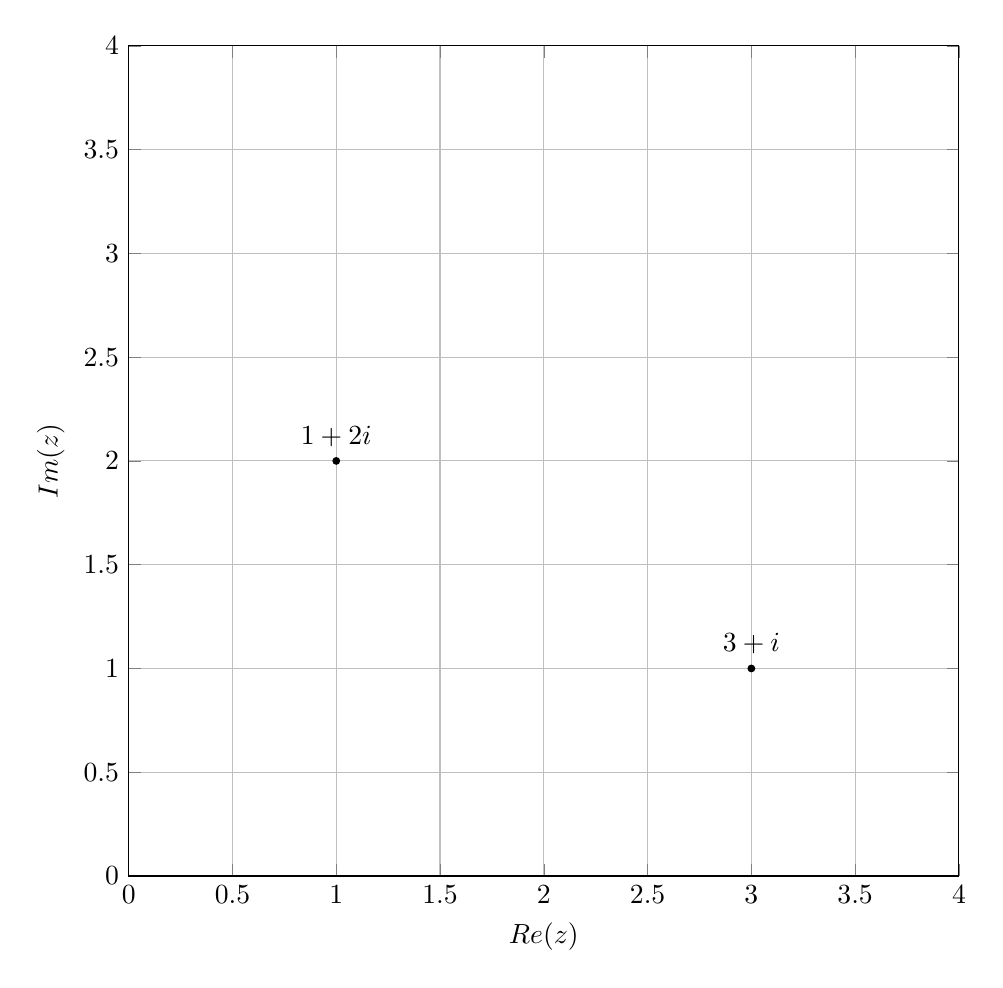
\begin{tikzpicture}
		\begin{axis}[
				xmin=0,xmax=4,
				ymin=0,ymax=4,
				restrict y to domain = 0:4, domain=0:4, width=\textwidth, height=\textwidth, grid=major, samples=200,  ylabel=$Im(z)$, xlabel=$Re(z)$]
			\node [circle, fill= black, inner sep=1, label= $1+2i$] at (1,2){};
			\node [circle, fill= black, inner sep=1, label= $3 + i$] at (3,1){};
		\end{axis}
	\end{tikzpicture}
\end{minipage}
%
\begin{minipage}[t]{0.48\textwidth}
	\begin{itemize}
		\item L'asse y è detta asse immaginaria
		\item Un numero con parte i mmaginaria nulla è detto puro
	\end{itemize}
\end{minipage}

\subsection{Somme e differenze}
\bigbox{Dati $z= a+bi, \quad w = c + di \quad  \in \C$ la loro somma è data da:
	\[
		\left( a+c \right) + \left( b+d \right) i
	\] }
\subsection{Prodotto}
\bigbox{Si usa la proprietà distributiva per il fatto che $i^2 = -1$ \[
		z * w = \left( a + bi \right) \left( c + di \right) = ac + adi + bci + bd \underbrace{i^2}_{=-1}
	\] }
\subsection{Reciproco}
\bigbox{Dato un numero $ z  \in  \C$, al fine di calcolarne il reciproco $ \frac{1}{z}$ posso razionalizzare, in modo da ottenere un numero in forma cartesiana
	\[
		\frac{1}{z} = \frac{1}{a + bi}= \frac{1}{a+bi} \frac{a-bi}{a-bi}= \frac{a-bi}{a^2+ b^2}
	\] }
\subsection{Divisione}
\bigbox{
	Per effettuare una divisione fra numeri complessi trovo il reciproco del divisore e effettuo la divisione
	\[
		\frac{c + di}{a + bi}= \frac{\left( ca + bd \right) }{a^2 + b^2} + \frac{ad - ^3 }{a^2 + b^2}i
	\]
}
\subsection{Definizioni}
\definizione{Numeri coniugati}{
	Dato $z = a + bi$ si dice coniugato di z e si indica con $ \overline{z} $ un numero uguale a \[
		a - bi
	\]
}
\begin{itemize}
	\item $z * \overline{z} = \left( a+bi \right) \left( a-bi \right)  = a^2 + b^2= \left|z\right|^2$ quindi ho come conseqguenza che $\frac{1}{z}= \frac{\overline{z}}{\left|z\right|^2}$
	\item
\end{itemize}
\definizione{Modulo numero complesso}{Dato $z = a + bi$ si dice il modulo di $z$ il numero \[
		\left|z\right| = \sqrt{a^2 + b ^2}
	\] }

\section{Rappresentazione trigonometrica}
\bigbox{
	Posso rappresentare il numero complesso $z = a + bi$ tramite coordinate polari, ossia angolo e distanza dall'origine
}
Ad esempio, per un $z  \in  \C $ che dista $\rho$ dall'origine e con l'asse x crea un angolo di $ \theta$ so che questo numero avra coordinate cartesiane
\[
	\rho \cos \theta + \rho \sin \theta
\]
Se invece ho un $ z  \in  \C$ di coordinate polari $\rho \cos \theta + \rho \sin \theta $ la rappresentazione cartesiana è
\[
	\begin{cases}
		\arctan \left( \frac{b}{c} \right) \quad \text{ se } -\frac{\pi}{2} \theta \frac{\pi}{2}                           \\
		\arctan \left( \frac{b}{c} \right) + \pi \quad \text{ se } \theta < -\frac{\pi}{2} \text{ o }\theta >\frac{\pi}{2} \\
	\end{cases}
\]
\subsection{Argomento di un numero complesso}
\textbox{L'argomento di un numero complesso è l'angolo che questo formerebbe con l'asse x se rappresentato in coordinate polari}
\subsubsection{Prodotto in forma trigonometrica}
\[
	z = \rho\left( \cos \theta + \sin \theta \right) \quad w = r \left( \cos \alpha + \sin \alpha \right)
\]
\[
	z w = \cos\left( \theta + \alpha \right) + \sin \left(  \theta + \alpha \right)
\]
\subsubsection{reciproco in forma trigonometrica}
\[
	\frac{1}{z} = \frac{\overline{z}}{\left|z\right|^2} = \frac{\rho \left( \cos \left( -\theta \right) + \sin \left( -\theta \right)  \right) }{\rho ^2}=
\]

\subsubsection{Divisione in forma trigonometrica}
\[
	\frac{z}{w} = z * \frac{1}{w} = \ldots = \frac{\rho}{r}\left[ \cos\left( \theta - \alpha \right) + i \sin \left( \theta - \alpha \right)  \right]
\]
\subsection{Forma esponenziale}
\bigbox{
	Un numero complesso di coordinate polari $\left( \rho, \theta \right) $ è espresso nel seguente modo: \[
		z = \rho e ^{i \theta}
	\]
}
Formula di passaggio fra forma trigonometrica e esponenziale:
\[
	e ^{ i \theta} = \cos \theta + i \sin \theta
\]
\subsection{Potenza di un numero complesso}
Se $z = \rho \left(  \cos \theta + i \sin \theta \right) $
\[
	z^{n} = \rho ^{n} \left( \cos \left( n \theta \right)  + i \sin \left( n \theta \right)  \right)
\]
Se $z = \rho e^{ i \theta}$
\[
	z^{n} = \rho ^{n} e ^{ i n \theta}
\]
\textbf{Dimostrazione per induzione}
\[
	z^{n+1} = z \cdot z^{n} = z \left( \rho ^{n} \left( \cos \left( n \theta \right)  + i \sin \left( n \theta \right)  \right)  \right)  = \rho ^{ n+1 } \left\{\cos \left[  \left( n+1 \right)  \theta \right] + i \sin \left[  \left( n+1 \right)  \theta \right]  \right\}
\]
\subsubsection{Esempio potenza}
\[
	\left( 1 + i  \right) ^{6}
\]
\begin{itemize}
	\item Metodo 1 - faccio binomio di Newtoon - roba da matti
	\item Metodo 2 - passo a forma esponenziale $\rho = \sqrt{2} $, $\theta = \frac{\pi}{4}$ \[
		      z = \sqrt{2} e^{i \frac{\pi}{4}}
	      \]
	      \[
		      \left( 1 + i \right) ^{ 6} = \sqrt{2} e ^{ i \frac{\pi}{4}} = \sqrt{2} ^{6} e ^{ i \frac{\pi}{4}6} = 8 e ^{i \frac{3}{2} \pi} = -8 i
	      \]
\end{itemize}
\[
	\left( 1 + i \right) ^{ 6000}= 2^{3000} e ^{i \frac{\pi}{4}6000} = 2^{3000}
\]
\subsection{Radici dei numeri complessi}
\definizione{Radici dei numeri complessi}{
	Dato un numero complesso $a  \in  \C$, le radici complesse n-esimi sono tutti i numeri complessi $z  \in  \C$ tali che $z^{n} = a$
}
NB: se $ a \neq 0$ esistono sempre n numeri complessi $z$ che verificano l'equazione $ z ^{ n } = a$. Questi numeri coincidono con i vertici di un poligono regolare di n lati con centro nell'origine
\vskip3mm
Supponiamo che $a = r e ^{ i \phi}$ e $ z = \rho e ^{ i \theta}$.
\[
	z^{n} = a \rightarrow \rho^{ n} e ^{ i n \theta} = r e ^{i \phi}
\]
Per soddisfare uguaglianza devo avere:
\begin{itemize}
	\item Stesso modulo $\rho ^{n}= r$
	\item Stesso argomento $n \theta = \phi + 2k \pi \quad  k  \in  \Z$
\end{itemize}
ossia rispettivamente
\begin{itemize}
	\item $\rho = \sqrt[n]{r} $
	\item $\theta = \frac{\phi}{n} + 2 \pi \frac{k}{n}$
\end{itemize}
NB: ottengo valori diversi solo per $k  \in  \left[ 0, n-1 \right] $
\incomprensione{11.22.37}
\textbf{Esercizio}
\textit{Trova le radici seste di $-i$}


\begin{itemize}
	\item Ciò corrisponde a risolvere l'equazione \[
	z^{n} = -i
	\] 
	\item $-i= 1e^{\frac{3}{2}\pi}$
	\item Le soluzioni sono: 
\[
\begin{cases}
	\rho = 1 \\
	6 \phi =\left( \frac{3}{2} \pi  + 2k\pi \right) 
\end{cases}
\] 
\end{itemize}
%
\begin{center}
	\framebox{\includegraphics{Images/Radici complessi.pdf}}
\end{center}
\section{Il teorema fondamentale dell'algebra}
Per polinomi a coefficienti reali $P\left( x \right) $ sapevamo che:
\bigbox{ $P\left( x \right)  = c_n x ^{n} + c_{n-1} x ^{ n-1} \ldots + c_1 x ^{1} + c_0 \quad c_n  \in  \R$ polinomio di grado $n$ a coefficienti reali. Ha al massimo n soluzioni.}

\definizione{Radice di un polinomio}{Dato un polinomio a coefficienti complessi$\alpha  \in  \C$ si dice radice di  $P\left( z \right) $ se $P\left( \alpha \right) =0$}

\definizione{Molteplicità radice}{Si diche che $\alpha  \in  \C$ è una radice di $ P\left( x \right) $ di molteplicità $ \mu  \in  \N$ se é è divisibile per $\left( x-\alpha \right) ^{\mu}$}
Per un polinomio a coefficienti complessi devi ridefinire il teorema fondamentale dell'algebra:
\bigbox{
$P\left( x \right) = c_n x ^{n} + c_{n-1} x ^{ n-1} \ldots + c_1 x ^{1} + c_0 \quad c_n  \in \C$ polinomio di grano $n$ a coefficienti complessi. Ha \underline{esattamente} n soluzioni}
quindi
\teorema{Teorema fondamentale dell'algebra}{Ogni polinimio $ p\left( x \right) $ di grado $n$ a coefficienti complessi ha  \underline{esattamente n radici complesse} eventualmente contando le rispettive moltepliicità}
Ogni polinomio a coefficienti complessi può essere scritto come prodotto di fattori di grado 1 
\[
P\left( z \right) = a_k x ^{k}\ldots a_1 x + a_0 = a_n \left( z-\alpha_1 \right)^{\mu_1} \left( z-\alpha_2 \right) ^{\mu_2}
\]
dove $\alpha_1, \alpha_2 \ldots \alpha_n$ sono radici $  \in  \C$ di $ P\left( z \right) $

\teorema{Radici complesse coniugate}{Sia $ P\left( z \right) $ polinomio a coefficienti reali. Se $ z  \in  \C$ è radice di $ P\left( z \right) $ allora anche $\overline{z}$ è radice di $ P\left( z \right) $}
\begin{itemize}
	\item Se $ \alpha  \in  \C$ è radice di P anche $\overline{\alpha}$ è radice di P
	\item Se $\alpha  \in  \C$ è radice di P con moltepicità $\mu  \in  \N$ allora $ \overline{\alpha}  \in  \C$ è radice di P con molteplicità $\mu$
\end{itemize}

Dimostrazione:
\begin{itemize}
	\item $P\left( x \right)  = \sum_{k=0}^{n} a_k x^k \quad P\left( \alpha \right) = 0$ per hp.
	\item $P\left( \alpha \right)  = \sum_{k=0}^{n} a_k \alpha^k = 0$
	i
\end{itemize}
\incomprensione{09:48:11}
\bigbox{
Ogni polinomio reale di grado $ n$ è prodotto di fattori di grado $1$ e di fattori irreducibili di grado 2
\begin{itemize}
	\item I fattori di grado dure rappresentano coppie di radici complesse coniugate eventualmente con molteplicità
\end{itemize}
}
\incomprensione{10:00:29}

\section{Successione numeri reali}
\subsection{Frequenza variabili}

\definizione{Freqentemente}{Si dice che una variabile $ P_n$ + vera (o falsa) \underline{frequentemente} se + vera per infiniti valori di $n  \in \N$}
\definizione{Definitivamente}{Si dice che una variabile $P_n$ è \underline{definitivamente} se \[
\exists n_0  \in \N \text{ t.c. } \quad P_n \text{ vera } \forall n \ge n_0
\] }
NB: se una variabile è vera definitivamente lo è anche frequentemente. Ma non vale il contrario: \[
\left( -2 \right) ^2 \ge 7
\] 
\begin{itemize}
	\item Vera frequentemente
	\item Falsa frequentemente
	\item Non è ne vera ne falsa definitivamente
\end{itemize}
\subsection{Successione di numeri naturali}
\definizione{Successione di numeri naturali}{E una funzione in cui l'insieme iniziale sono i numeri \underline{naturali} e l'insieme finale sono i nueri \underline{reali} \[
f: \N \rightarrow \R
\]
il termine n-esimo della succesione si indica con $f_n$}
NB: la seguente non è una successione:
\[
a_n = \frac{1}{n-2022}
\] 
in quanto per $n=2022$ risulta $\frac{1}{0}$ che non è definito, per questo usiamo una definizione più accomodante
\definizione{Successione di numeri reali accomodante}{Consideriamo succeesione di numeri reali quelle che sono vere almento definitivamente, ossia che siano definite da un determinato indice $ n_0$ in poi}
Esempi:
\begin{itemize}
	\item $a_n = \frac{1}{n+5}$ \quad vera in senso classico
	\item $b_n= \frac{1}{n-5}$ \quad vera in senso accomodante per $n\ge 6$
	\item $c_n= \sqrt{n-2022} $ \quad vera in senso accomodante per $n \ge 2022$
	\item $b_n= \sqrt{2022-n} $ \quad non è una successione \rarr $\nexists n_0 \text{ t.c. }b_n \text{ vera } \forall n \ge n_0$
\end{itemize}
\subsection{Rappresentazione di successioni}
Posso rappresentare successioni come normali funzioni, quindi \underline{traite grafico}
\begin{itemize}
	\item \underline{Tramite grafico} \quad $\left( n, f\left( n \right)  \right) $ 
	\[
	f\left( n \right) = a_n = \frac{1}{n}
	\] 
	\begin{center}
		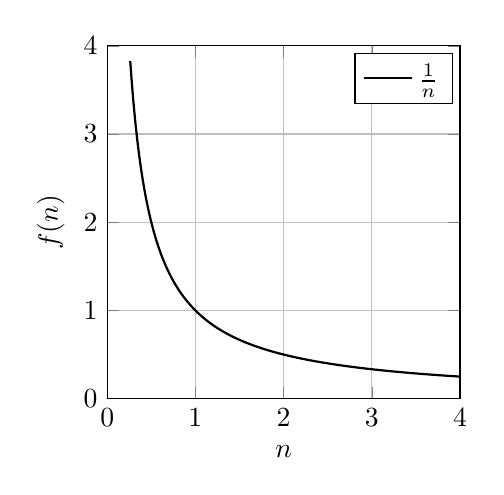
\begin{tikzpicture}
			\begin{axis}[
			xmin=0, xmax=4,
			ymin=0,ymax=4,
			restrict y to domain = 0:4, domain=0:4, width=0.5\textwidth, height=0.5\textwidth, grid=major, samples=200,  ylabel=$f(n)$, xlabel=$n$, legend entries={$\frac{1}{n}$}]
			\addplot[black, thick] {1/x};
			\end{axis}
		\end{tikzpicture}
	\end{center}	
	\item Sulla retta dei numeri reali:
	\begin{tikzpicture}
		\begin{axis}[
		axis y line = none,
		xmin=0, xmax=1,
		ymin=0,ymax=0,
		domain=0:1, width=0.5\textwidth, height=0.1\textwidth]
		\coordinate (zero) at (1,0){};
		\coordinate (uno) at (1/2,0){};
		\coordinate (due) at (1/3,0){};
		\coordinate (tre) at (1/4,0){};
		\coordinate (quattro) at (1/5,0){};
		\end{axis}
		\node [fill = black, circle, inner sep = 1pt, label = north: $1$] at (zero){};
		\node [fill = black, circle, inner sep = 1pt, label = north: $\frac{1}{2}$] at (uno){};
		\node [fill = black, circle, inner sep = 1pt, label = north: $\frac{1}{3}$] at (due){};
		\node [fill = black, circle, inner sep = 1pt, label = north: $\frac{1}{4}$] at (tre){};
		\node [fill = black, circle, inner sep = 1pt, label = north: $\frac{1}{5}$] at (quattro){};
	\end{tikzpicture}
	\item Rapppresentazione dinamica: i mmagino di accendere una lampadina ogni tot secondi e in corrispondenza dell'accensione segno il valore della funzione
\end{itemize}

\subsection{Limite di una successione}
\label{sub:tipilimiti}
Una successione ha 4 possibilità:
\begin{itemize}
	\item $\lim_{n \to \infty} a_n = l \in  \R$ ossia $a_n \to l$
	\begin{itemize}
		\item $\lim_{n \to \infty} a_n = l^{+}$ ossia ha $a_n \ge l$ \underline{definitivamente} 
		\item $\lim_{n \to \infty} a_n = l^{-}$ ossia $a_n \le l$ \underline{definitivamente}
		\item $\lim_{n \to \infty} a_n = l$ oscillando intorno al valore
	\end{itemize}
	\item $\lim_{n \to \infty} a_n = + \infty$ ossia $a_n \to \infty$ 
	\item $\lim_{n \to \infty} a_n = - \infty$ ossia $a_n \to -\infty$
	\item $\lim_{n \to \infty} a_n \quad \text{ NON esiste }$ ossia $a_n$ non ha limite
\end{itemize}
Definizione formale di limite
\definizione{Limite infinito}{Si diche che $a_n \to + \infty$ se \[
\forall M \in  \R \exists a_m \text{ t.c. } a_m\ge M
\] 
ossia $a_m \ge M$ \underline{definitivamente}
\vskip3mm
Si dice che $a_n \to -\infty$ se \[
\forall M \in  \R \exists a_m \le M 
\] 
ossia $a_m \ge M $}

\definizione{Limite se tenda a numero finito}{Si dice che $a_n \to l \in  \R$ \[
 \forall \epsilon \ge 0 \quad l- \epsilon \le a_n \le l+ \epsilon
\] 
ossia 
\[
\left|a_n-l\right| \le \epsilon \quad \text{ \underline{definitivamente} }
\] }

\subsubsection{Errori comuni}
\begin{itemize}
	\item Se $a_n \to \infty$ allora è definitivamente crescente. NO: potrei avere una successione che somma 2 e scende di 1 all'infinito
	\item Se $a_n \to 0$ allora tende o a $0^{+}$ o a $0^{-}$. NO: vedi $\frac{\left( -1 \right) ^{n}}{n}$
	\item Se $a_n$ non è limitata superiormente allora $a_n \to \infty$. NO: vedi $ \left( -2 \right) ^{n}$
\end{itemize}
\subsection{Esempi}
\underline{Esempio 1}
\[
a_n = n^2
\] 
Dimostriamo che $a_n \to \infty$
2 casi:
\begin{itemize}
	\item Se $M \le 0 $ \rarr $ n^2 \ge M$ sempre
	\item Se $M \ge 0 $ \rarr $n^2 \ge M \Leftrightarrow n \ge \sqrt{M} $
\end{itemize}
\underline{Esempio 2}
\[
a_n = \sqrt{n} 
\] 
Dimostriamo che $a_n \to \infty$ 2 casi:
\begin{itemize}
	\item Se $M \le 0 $ \rarr $\sqrt{n} \ge M$ sempre
	\item Se $M \ge 0$ \rarr $\sqrt{n} \ge M \Leftrightarrow n \ge M^2$
\end{itemize}
\bigbox{
\[
\lim_{n \to \infty} n ^{a} = \infty \quad \forall a\ge 0 
\]
}
\underline{Esemipio 3}
\[
\lim_{n \to \infty} \frac{1}{n} = o^{+} 
\] 
Devo verificare che \[
\forall \epsilon > 0 \quad 0 < \frac{1}{n} \ge \epsilon
\] 
\begin{itemize}
	\item $a < \frac{1}{n}$ definitivamente in quanto $n$ è naturale
	\item $\frac{1}{n} \le \epsilon \Leftrightarrow \frac{1}{\epsilon} \le n$
\end{itemize}
\bigbox{
\[
\lim_{n \to \infty}  n ^{\alpha} =0 \quad \forall \alpha \le 0
\] 
}

\teorema{Permanenza del segno}{Se $a_n \to l > 0$ allora $a_n > 0 $ definitivamente\\
Se $a_n \to l<0$ allora $a_n < 0 $ definitivamente}
\underline{Dimostrazione}

\subsection{Unicità del limite}
Una successione ha sempre \underline{solo uno } dei comportamenti descritti in subsec \ref{sub:tipilimiti}
\underline{Dimostrazione}

\begin{itemize}
	\item Supponiamo che uno stesso limite tenda a due cose diverse $a_n \to l_1$ e $a_n \to l_2$ con $l_1 \neq l_2$
	\item Per la definizione di limite il valore del limite deve ricadere in un intorno di $l_1$ e $ l_2$. Se questi due intervalli sono sufficientemente piccoli e dunque non hanno punti in comune dovrei \underline{avere un punto che sta in due parti contemporaneamente}. Ne concludiamo che l'ipotesi sia falsa
\end{itemize}
\subsection{Teoremi sui limiti}
\label{sub:teoremilimiti}
\teorema{Teorema del confronto a 2}{Siano $a_n $ e $b_n$ succesioni. Supponiamo che $a_n \ge b_n$ almeno definitivamente
\begin{itemize}
	\item Se $b_n \to \infty$ allora $a_ n \to \infty$
	\item Se $a_n \to -\infty$ allora $b_n  \to -\infty$
\end{itemize}}
\label{teoconfrontoadue}
\teorema{Teorema del confronto a 3 (dei due carabinieri)}{Siano $a_n, b_n, c_n$ successioni tali che $a_n \le b_n \le c_n$ almeno definitivamente. Supponiamo che $a_n \to l \in  \R$ e $c_n \to l \in  \R$ allora $ b_n \to l \in  \R$}
\label{teoconfrontoatre}
\subsection{Errori comuni}
\begin{itemize}
	\item Supponiamo che a $a_n > b_n$ e $a_n \to l_1, b_n \to l_2$. Allora \[
	l_1 > l_2
	\] 
	\item \underline{Falso} in quanto al limite non si conserva l'uguale. Vedi ad esempio:
	\[
	a_n = \frac{2}{n} \quad b_n = \frac{1}{n}
	\] 
	nonostante i termini di $a_n$ siano sempre il doppio di quelli di $ b_n$ il loro limite è lo stesso e vale 0. Posso in caso affermare che se $a_n > b_n$ allora $l_1 \ge l_2$
\end{itemize}

\subsection{Retta reale estesa}
\label{sub:rettarealeestesa}
\[
\overline{\R} = \R \cup \left\{ +\infty \right\} \cup \left\{ - \infty \right\} 
\] 
\teorema{Somma, prodotto e divisione limiti}{Siano $a_n$ e $b_n$ successioni reali. \[
a_n \to l_1 \in  \R \text{ e } b_n \to l_2 \in  \R
\] 
allora 
\begin{align*}
a_n + b_n &\to l_1 + l_2 & a_n - b_n &\to l_1-l_2\\
a_n b_n & \to l_1l_2 & \frac{a_n}{b_n} &\to \frac{l_1}{l_2}\\
a_n^{b_n} & \to l_1^{ l_2}
\end{align*}

A meno che non si cada in uno di questi 7 casi speciali:
\begin{gather*}
	+\infty - \infty \quad 0 \cdot \left( \pm \infty \right) \frac{0}{0} \quad  \frac{\pm \infty}{\pm \infty}\\
\quad 0^{0} \quad \left( + \infty \right) ^{0} \quad 1^{\pm \infty}\\
\end{gather*}
}
NB: nel caso della successione di tipo $\frac{a_n}{b_n}$ devo stare attento al modo in cui $b_n$ tende a zero: può tendere a $a^{+}, 0 ^{-}$ o a $0$

\subsection{Forma indeterminata}
\textbf{Esempio 1}
\[
a_n = \underbrace{n^3}_{+ \infty} + \underbrace{n^2}_{+\infty} \to + \infty
\] 
\textbf{Esempio 2}
\[
a_n = \underbrace{n^3}_{+ \infty} -  \underbrace{n^2}_{+\infty} = \underbrace{n^2}_{\infty} \underbrace{\left( n-1 \right)}_{+\infty-1}  \to + \infty
\] 
\textbf{Esempio 3}
\[
a_n= \underbrace{\sqrt{n}}_{+\infty} - \underbrace{\frac{1}{n^3}}_{0} \to + \infty
\]
\textbf{Esempio 4}
\[
a_n = 2^{n}
\] 
Dimostro con \underline{disuguaglianza di Bernoulli}(sub \ref{sub:disbernoulli}):
\[
2^{n} \ge n+1
\] 
dunque visto che $ n+1 \to \infty$ allora anche $2^{n} \to \infty$ per \underline{teorema del confronto a 2}(teo \ref{teoconfrontoatre})

\textbf{Esempio 5} 
\[
\lim_{n \to \infty} \frac{\arctan \left( 2^{n} + n! \right) }{n^2 + 3} = 0
\] 
\[
\lim_{n \to \infty} \frac{\sin\left( n \right)}{n}  = 0
\] 
in quanto al numeratore ho valoni finiti e al demonimatore valori infiniti. Posso applicare teorema dei dure carabinieri:
\begin{itemize}
	\item $0 \le \arctan \left( 2^{n} + n! \right) \le \pi$
	\item Diviso per $ n^2 + 3$
	\[
	0 \le \frac{\arctan \left( s^{n} + n! \right) } {\underbrace{n^2 + 3}_{\to 0}} \le \frac{\pi}{\underbrace{n^2 + 3}_{\to 0}}
	\]
	\item Il mio limite deve essere compreso fra $0$ e $0$, quindi è $=0$ per il teorema del confronto a tre (teo \ref{teoconfrontoatre})
\end{itemize}
\textbf{Esempio 6}
\[
\lim_{n \to \infty} \frac{\sqrt{n} - \sqrt[3] {n} }{n + 10^{23}} = \frac{n^{\frac{1}{2}}\left( 1- n^{-6} \right)}{n}  = \frac{1}{\sqrt{n} }\left( 1-n^{-6} \right) \to 0
\] 
\subsection{Implicazione i mportante disuquaglianza di bernoulli}
Dimostro che 
\[
\lim_{n \to \infty} a ^{ n} = + \infty \quad \forall a > 1
\] 
\begin{itemize}
	\item Noto che 
	\[
	a^{n}= \left( 1 + \left(  a-1 \right)  \right) ^{n}
	\] 
	\item questa quantità per il teorema di bernoulli è maggiore di:
	\[
	\left( 1 + \left( a-1 \right)  \right) ^{n} \ge 1 + n\left( a-1 \right) 
	\] 
	\item Se $a > 1$ $\lim_{n \to \infty} n\left( a-1 \right) = + \infty $
\end{itemize}
Se invece ho $a \in  \left( 0,1 \right) $
\[
\lim_{n \to \infty} a^{n} \quad \text{  con  }a \in  \left( 0,1 \right)  
\]
Visto che $a \in  \left( a,1 \right) $ posso supporre che $a=\frac{1}{b}$ con $b > 1$
\[
a^{n} = \left( \frac{1}{b} \right) ^{n} = \frac{1}{b^{n}} \to 0
\] 
\section{Fattoriali e combinatoria}
\definizione{Fattoriale di un numero}{Il fattoriale di un numero è definito nel seguente modo:
\[
0! = 1
\] 
\[
\left( n+1 \right) ! = \left( n+1 \right) \cdot n!
\] 
in numeri $ n!$ rapprentenza il numero di modi in cui posso ordinare $n$ oggetti
}
Per scegliere n persone posso pensare che 
 \begin{itemize}
	\item La prima persona la posso scieglere in $n$ modi
	\item La seconda in $n-1$
	\item La terza in $n-2$
	\item \ldots la k esima in $n-k+1$
\end{itemize}
quindi
\begin{table}[h!]
	\centering
	\begin{tabular}{|c|c|c|c|c|}
	\hline
	n & n-1 & n-2 & \ldots & n-k+1 \\
	\hline
	\end{tabular}
\end{table}

\definizione{Coefficiente binomiale}{
Dati 2 interi $n,k \quad 0 \le k\le n$, ponto \[
\binom{n}{k}= \frac{n!}{k! \left( n-k \right) !}
\]  
}
Immagino di avere un esercito di $n$ soldati e ne devo estrarre k. Non conta l'ordine con cui gli estraggo
\begin{itemize}
	\item Il primo soldato lo posso scegliere in $n$ modi
	\item Il secondo in $n-1$
	\item Il terzo in $n-2$
	\item \ldots il k esimo in $n-k+1$
	\item Devo poi dividere per il le permutazioni possibili visto che \underline{l'ordine non conta}
	\[
	\text{ numero modi di estrarre } = \frac{n\left( n-1 \right) \left( n-2 \right) \ldots \left( n-k+1 \right)}{k!} = \binom{n}{k}
	\] 
	\item Perchè diviso? Pensa al fatto che ogni squadra estratta può essere disposta in $k!$ modi, quindi $k!$ modi vanno considerati come la stessa squadra
\end{itemize}
\subsection{Proprietà dei fattoriali}
\begin{itemize}
	\item Scontate:
	\begin{align*}
	\binom{n}{0} &=  \frac{n!}{0!n!}= 1 &  \binom{n}{n}&=  \frac{n!}{n!0!}= 1 \\
	\binom{n}{1} &=  \frac{n!}{1!\left( n-1 \right) !}=  \frac{n \left( n-1 \right) !}{\left( n-1 \right) }=n &  \binom{n}{n-1} &= \frac{n!}{\left( n-1 \right) 1!}= \frac{n\left( n-1 \right) !}{\left( n-1 \right) !}=n
	\end{align*}
	\item Simmetrica: prendere $k$ persona da squadra di $n$ è la stessa cosa che lasciarne fuori $n-k$ :
\[
\binom{n}{k}= \binom{n}{n-k}
\] 
	\item Generazione ricorsiva binomiale:
	\[
	\binom{n+1}{k+1} = \binom{n}{k} + \binom{n}{k+1}
	\]
	Dimostrazione
		\begin{align*}
		\binom{n}{k} + \binom{n}{k+1} &=  \frac{n!}{k! \left( n-k \right) !} + \frac{n!}{\left( k+1 \right) \left( n-k-1 \right) !}\\
		&= \frac{n!}{k! \underbrace{\left( n-k \right)}_{\left( n-k \right) \left( n-k-1 \right) !} !} + \frac{n!}{\underbrace{\left( k+1 \right)}_{\left( k+1 \right) k!} \left( n-k-1 \right) !} \\
		&= \frac{n!}{k! \left( n-k-1 \right) !} \frac{k+1 +n-k}{\left( n-k \right) \left( k+1 \right) }
		\end{align*}
A livello combinatorio
\begin{itemize}
	\item Prendo un gruppo di $n$ persone e tengo separatamente 1
	\item Per formare un gruppo grande $k+1$ posso:
	\begin{enumerate}
		\item Creare un gruppo grande $n$ e poi aggiungerci il nuovo arrivato
		\item Creare un gruppo grande $n+1$ che non contenga il nuovo arrivato 
	\end{enumerate}
	\item Nel primo caso posso creare $ \binom{n}{k}$ gruppi
	\item nel secondo caso posso create $ \binom{n}{k+1}$ gruppi
\end{itemize}
\end{itemize}
\subsection{Il triangolo di tartaglia}
	\begin{center}
		\includegraphics{Images/Tartaglia.pdf}
	\end{center}
Ogni valore è dato dalla somma dei valori dei termini \underline{sopra} di esso a \underline{sinistra e a destra}
\bigbox{Il coefficiente alla riga n nella posizione k è dato da \[
\binom{n}{k}
\] 
visto che il coefficiente nella posizione $n+1, k+1$ è uguale al coefficiente nella posizione $n, k$ e $n, k+1$ noto che questo triangolo verifica la generazione ricorsiva binomiale:
\[
\binom{n+1}{k+1}= \binom{n}{k} + \binom{n}{k+1}
\]
}
\bigbox{
Nello sviluppo di un binomio del tipo $\left( x+y \right) ^{n}$ il monomio $x^{k}y^{n-k}$ ha coefficiente $ \binom{n}{k}$ ossia:
\[
\left( x+y \right) ^{n} = \sum_{k=0}^{n} \binom{n}{k}x^{k}y^{n-k}
\] 
}
\bigbox{
La somma dei coefficienti alla riga $n$ è uguale a \[
2^{n}
\] 
}

Dimostrazione:
\begin{itemize}
	\item Applico sviluppo del binomio $\left( x+y \right) ^{n}$ con $x=y=1$
	\item In questo caso so che \[
	\left( 1+1 \right) ^{n} = 2^{n}= \sum_{k=0}^{n} \binom{n}{k}1^{k}1^{n-k}= \sum_{k=0}^{n} \binom{n}{k}
	\] 
\end{itemize}
\section{3 criteri: rapporto, radice, rapporto-radice}
\subsection{Criterio della radice}
\begin{itemize}
	\item Sia $a_n$ una successione tale che $a_n \ge 0 $ definitavente
	\item Supponiamo che se $\sqrt[n]{a_n} \to l \in  \R \cup \left\{ +\infty \right\} $ allora ho 3 possibilità:
	\begin{itemize}
		\item se $l > 1$, allora $ a_n \to +\infty$
		\item se $l < 1$, allora $a_n \to 0$
		\item se  $l=1$ il criterio non fornisce informazioni 
	\end{itemize}
\end{itemize}
\subsection{Criterio del rapporto}
\begin{itemize}
	\item Sia $a_n$ una successione tale che $a_n > 0$ definitivamente
	\item Supponiamo che $\lim_{n \to \infty} \frac{a_n+1}{a_n}=l \in  \R \cup    \left\{ +\infty \right\} $
	allora ho 3 possibilità
	\begin{itemize}
		\item se $l > 1$, allora $ a_n \to +\infty$
		\item se $l < 1$, allora $a_n \to 0$
		\item se  $l=1$ il criterio non fornisce informazioni 
	\end{itemize}
\end{itemize}
\subsection{Criterio rapporto $ \rightarrow $ radice}
\begin{itemize}
	\item Sia $a_n$ una successione tale che $a_n > 0 $ definitivamente
	\item Supponiamo che $\frac{a_{n + 1}}{a_n} \to l \in  \R \cup \left\{ +\infty \right\} $
allora
\[
\sqrt[n]{a_n} \to l
\] 
ossia $\frac{a_{n +1}}{a_n}$ e $\sqrt[n]{a_n} \to l$ tendono allo stesso $l \in \R \cup \left\{ +\infty \right\} $
\end{itemize}
\subsection{Dimostrazioni}
\subsubsection{Dimostrazione criterio radice}
\begin{itemize}
	\item Prendo punto a metà fra 1 e $l$
	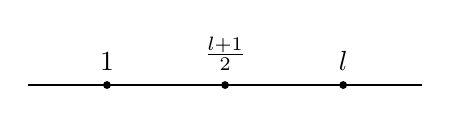
\begin{tikzpicture}
			\node [label=north: 1 , fill=black, circle, inner sep = 1pt] at (0,0) {};
			\node [label=north: $l$ , fill=black, circle, inner sep = 1pt] at (3,0) {};
			\node [label=north: $\frac{l+1}{2}$ , fill=black, circle, inner sep = 1pt] at (1.5,0) {};
			\draw (-1,0) to (4,0);
	\end{tikzpicture}
	\item Visto che $\sqrt[n]{a_n} \to l$ necessariamente 
	\[
	\sqrt[n]{a_n} \ge \frac{l+1}{2}
	\] 
	\item Ho quantità positive sia a sinistra che a destra, posso elevare alla $n$ da entrambe le parti, ottenendo:
\[
a_n \ge \left( \frac{l+1}{2} \right) ^{n}
\] 
	\item Se $l > 1$ $\left( \frac{l+1}{2} \right)^{n}  \to \infty$
\end{itemize}
\hr
se invece $l<1$ agisco nello stesso modo:
\begin{itemize}
	\item Prendo punto a metà fra $l$ e 1
	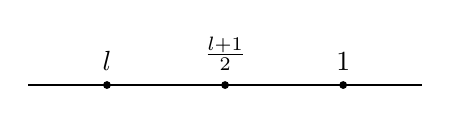
\begin{tikzpicture}
			\node [label=north: 1 , fill=black, circle, inner sep = 1pt] at (3,0) {};
			\node [label=north: $l$ , fill=black, circle, inner sep = 1pt] at (0,0) {};
			\node [label=north: $\frac{l+1}{2}$ , fill=black, circle, inner sep = 1pt] at (1.5,0) {};
			\draw (-1,0) to (4,0);
	\end{tikzpicture}
	\item Visto che $\sqrt[n]{a_n} \to l$ necessariamente 
	\[
	\sqrt[n]{a_n} \le \frac{l+1}{2}
	\] 
	\item Ho quantità positive sia a sinistra che a destra, posso elevare alla $n$ da entrambe le parti, ottenendo:
\[
a_n \le \left( \frac{l+1}{2} \right) ^{n}
\] 
	\item Se $l < 1$ $\left( \frac{l+1}{2} \right)^{n}  \to 0$
	\item Siccome $a_n \ge 0$ per ipotesi allora 
	\[
	0 \le a_n \le \left( \frac{l+1}{2} \right) ^{n}
	\] 
	ossia $a_n \to 0$ per teorema del confronto a tre
\end{itemize}
\subsection{Numero di nepero}
\bigbox{
Il numero di nepero è definito dal seguente limite
\[
\lim_{n \to \infty} \left( 1+\frac{1}{n} \right) ^{n} 
\] 
}
\subsection{Esempio forme indeterminate}
\textbf{Esempio 1}
\[
\lim_{n \to \infty} \frac{n^{n}}{n!} = + \infty
\]
Criterio del rapporto:
\[
\frac{a_{n+1}}{a_n} = \frac{\left( n+1 \right) ^{n+1}}{\left( n+1 \right) !} \cdot\frac{n!}{n^{n}}
\] 
\textbf{Esempio 2}
\[
\lim_{n \to \infty} \frac{3^{n^{2}}}{n!} = +\infty
\]
Criterio del rapporto:
\[
\frac{a_{n+1}}{a_n} = \frac{3^{\left( n+1 \right) ^{2}}}{\left( n+1 \right) !}
\] 
\textbf{Esempio 3}
\[
\lim_{n \to \infty} \frac{\sqrt[n]{n!} }{n} = 
\] 
Criterio rapporto radice
\[
\frac{\sqrt[n]{n!} }{n} = \sqrt[n]{\frac{n!}{n^{n}}} 
\]
\section{Limiti di funzioni}
\definizione{Limite di funzione}{
Data una funzione $f : A \rightarrow \R \quad  A \subseteq \R$ abbiamo tre tipologie di limite:
\[
\lim_{x \to \infty} f(x) \quad \lim_{x \to -\infty} f(x) \quad \lim_{x \to x_0} f(x)  
\] 
\textbf{Primo tipo:}
\[
\lim_{x \to \infty} f(x) = \begin{cases}
	l \in \R\\
	+ \infty \\
	- \infty \\
	\text{ non esiste }
\end{cases}
\] 
se $ \lim_{x \to \infty} f(x) = + \infty$: 
\[
\forall M \in  \R \quad \exists k \in  \R \text{ t.c. } f\left( x \right) \ge M \forall x \ge k
\] 
se $ \lim_{x \to \infty} f(x) = + -\infty$: 
\[
\forall M \in  \R \quad \exists k \in  \R \text{ t.c. } f\left( x \right) \le M \forall x \ge k
\] 
se $ \lim_{x \to \infty} f(x) = l$: 
\[
\forall \epsilon > 0 \quad \exists k \in  \R \text{ t.c. } l- \epsilon \le f\left( x \right) \le l+ \epsilon \quad \forall x \ge k
\] 
ossia 
\[
\left|f\left( x \right) -l\right| \le \epsilon
\] 
se $ \lim_{x \to \infty} f(x) = l^{+}$: 
\[
\forall \epsilon > 0 \quad \exists k \in  \R \text{ t.c. }  l <  f\left( x \right) \le l+ \epsilon \quad \forall x \ge k
\] 
se $ \lim_{x \to \infty} f(x) = l^{-}$: 
\[
\forall \epsilon > 0 \quad \exists k \in  \R \text{ t.c. }  l-\epsilon \le f\left( x \right) \le l \quad \forall x \ge k
\] 
\textbf{Secondo tipo}: molto simile a primo, semplicemnte speculare
\vskip3mm
\textbf{Terzo tipo:}
\[
\lim_{x \to x_0} f(x) =
\begin{cases}
	l \in  \R \\
	+ \infty\\
	-\infty
	\text{ non esiste }
\end{cases}
\]
se $\lim_{x \to x_0} f(x) = + \infty$:
\[
\forall M \in  \R \quad \exists \delta > 0 \text{ t.c. } f\left( x \right)  \ge M \quad \forall x \in \left[ x_0-\delta, x_0+\delta \right] \setminus \left\{ x_0 \right\}  
\] 
se $\lim_{x \to x_0} f(x) = l \in  \R$:
\[
\forall \epsilon >0 \quad \exists \delta > 0 \text{ t.c. } \left|f\left( x \right) -l \right|\le \epsilon \text{ se } x \in \left[ x_0- \delta, x_0+ \delta \right] \setminus \left\{ x_0 \right\} 
\] 
}
\subsection{Continuità}
\definizione{Continuità}{
Una funzione $ f: A \rightarrow \R \text{ con } A \subseteq \R$ si dice continua in un punto $x_0 \in  A$ se:
\[
\lim_{x \to x_0} f(x) = f\left( x_0 \right) 
\] 
}
OSS:
\begin{itemize}
	\item Si dice che $f$ è continua in $A$ se essa è continua in ogni punto di $A$
	\item Le funzioni elementari sono sempre comtinue sul loro dominio
	\item Se faccio operazioni algebriche su funzioni continue ottengo funzioni continue
	\item La composizione di funzioni continue è continua
\end{itemize}
\subsection{Limiti notevoli}
Limiti "nonni"
\begin{gather}
	\lim_{x \to 0} \frac{\sin\left( x \right) }{x} = 1 \\
	\lim_{x \to + \infty} \left( 1+\frac{1}{x} \right) ^{x} = e
\end{gather}
Limiti "di seconda generazione"
\begin{align*}
	& \lim_{x \to 0} \frac{1-\cos\left( x \right) }{x^2} = \frac{1}{2} &\lim_{x \to 0} \frac{e^{x}-1}{x}=1 \\
	& \lim_{x \to 0} \frac{\log\left( 1+x \right) }{x}=1 &\lim_{x \to -\infty} \left( 1+\frac{1}{x} \right) ^{x} = e\\
	& \lim_{x \to 0} \frac{ \tan \left( x \right) }{x}=1  & \lim_{x \to 0} \frac{\arctan \left( x \right) }{x} = 1  \\
	& \lim_{x \to 0} \frac{\arcsin \left( x \right) }{x} = 1 & \lim_{x \to 0} \frac{a^{x}-1}{x}= \log \left( a \right) \\
	& \lim_{x \to 0^{+}} x \log \left( x \right) =0
\end{align*}
\subsection{Cambio di variabile}
\textbf{Esempio 1} 
\[
\lim_{x \to 0} \frac{\sin\left( x^2 \right) }{x^2} 
\] 
pongo $y=x^2$ 
\[
\lim_{x \to 0} \frac{\sin\left( x^2 \right) }{x^2}= \lim_{y \to 0} \frac{\sin\left( y \right) }{y}= 1 
\] 
\textbf{Esempio 2}
\[
\lim_{x \to  0} \frac{e^{\sin\left( x \right) }-1}{\sin\left( x \right) } 
\] 
pongo $y=\sin\left( x \right) $ ; se $x \to 0 \Rightarrow \sin\left( x \right) \to 0 \Rightarrow y \to 0$ 
\[
\lim_{x \to 0} \frac{e^{\sin\left(  \right) -1}}{\sin\left( x \right) }= \lim_{y \to 0} \frac{e^{y}-1}{y}  
\] 
\textbf{Esempio 3}
\[
\lim_{x \to \pi } \frac{\log\left( 1+\sin\left( x \right)  \right) }{\sin\left( x \right) } 
\] 
pongo $y=\sin\left( x \right) $ ; se $x \to \pi \Rightarrow \sin\left( x \right) \to 0 \Rightarrow y \to 0$
\[
\lim_{x \to \pi } \frac{\log\left( 1+\sin\left( x \right)  \right) }{\sin\left( x \right) } = \lim_{y \to 0} \frac{\log \left( 1+y \right) }{y} 
\] 
\textbf{Esempio 4}
\[
\lim_{x \to 0} \frac{1-\cos\left( x \right) }{x^2} 
\]
moltiplico e divido per $1+\cos\left( x \right) $ 
\[
\lim_{x \to 0} \frac{1-\cos\left( x \right) }{x^2} = \lim_{x \to 0} \left(\frac{1-\cos\left( x \right) }{c^2} \cdot \frac{1+ \cos \left( x \right) }{1 + \cos \left( x \right) } \right) = \lim_{x \to 0} \frac{1-\cos ^2 \left( x \right) }{x^2} \cdot \frac{1}{1+\cos\left( x \right) }  = 
\]
\[
=\lim_{x \to 0} \left( \frac{\sin \left( x \right) }{x} \right) ^2 \cdot \frac{1}{1+\cos\left( x \right) } = 1 \cdot \frac{1}{2}
\]
\textbf{Limite}
\[
\lim_{x \to 0} \frac{e^{x} -1}{x}
\] 
pongo $ x = \log \left( y+1 \right) $ 
\[
 \lim_{y \to 0} \frac{y}{\log \left( 1+y \right) }  = \lim_{x \to 0} \frac{1}{\underbrace{\frac{\log\left( 1+ y\right) }{y}}_{\text{limite notevole}}} 
\] 
\textbf{Limite}
\[
\lim_{x \to 0} \frac{e^{x}-1}{x} 
\] 
pongo $a^{x}=x \log \left( a \right) $
\[
\frac{e^{x \log \left( a \right)  }}{x} \cdot  
\] 
\subsection{Ordini di infiniti}
\bigbox{
\[
\lim_{x \to \infty} \frac{\left( \log \left( x \right)  \right) ^{a}}{x^{b}}=0 \quad \forall e>0, b>0
\] 
}
dimostro facendo cambiodi variabile (im pongo $y= \log \left( x \right) $)
\bigbox{
\[
\lim_{x \to 0^{+}} x \log \left( x \right) = 0
\] 
}
pongo $y=\frac{1}{y}$

\subsection{Dimostrazioe $\lim_{x \to 0} \frac{\sin\left( x \right) }{x} $}
\begin{itemize}
	\item Sappaimo che vale la seguente disuguaglianza:
	\[
	\sin \left( x \right) \le x \le \tan \left( x \right) 
	\] 
	\item Divido per $\sin\left( x \right) $
	 \[
	 1 \le \frac{x}{\sin\left( x \right) }\le \frac{1}{\cos\left( x \right) }
	 \] 
\end{itemize}
\subsection{Altri esempi}
\textbf{Esempio 1}
\[
\lim_{x \to  0} \frac{\log \left( \cos \left( x \right)  \right) }{x^2}  
\]
\begin{itemize}
	\item
	\[
\lim_{x \to  0} \frac{\log \left( \cos \left( x \right)  \right) }{x^2}  = \lim_{x \to 0} \frac{\log\left( \cos \left( x \right) +1 -1 \right) }{x^2} 
	\] 
	\item Moltiplico e divito per $\cos\left( x \right) -1$
	\[
	\lim_{x \to 0} \frac{\log \left( 1+ \left( \cos \left( x \right) -1 \right)  \right) }{\cos \left( x \right) -1} \cdot \frac{\cos \left( x \right) -1}{x^2} 
	\] 
	\item Ottengo due limiti notevoli
\end{itemize}
\textbf{Esempio 2}
\[
\lim_{x \to 0} \left( \cos\left( x \right) \right) ^{\frac{1}{x^2}}  
\] 
\begin{itemize}
	\item Ricordo che $A^{B}=e^{B\log A}$
	\item 
	\[
\lim_{x \to 0} \left( \cos\left( x \right) \right) ^{\frac{1}{x^2}}  = \lim_{x \to 0} e^{\frac{1}{x^2}\log\left( \cos\left( x \right)  \right) } 
	\] 
\end{itemize}
\textbf{Esempio 3}
\[
\lim_{x \to 0} \frac{e^{\tan \left( x \right) }- \cos\left( x \right) + \arctan \left( 2x \right) }{x} 
\]
\begin{itemize}
	\item Sommo e sottraggo 1
\[
\lim_{x \to 0} \frac{e^{\tan \left( x \right) }-1 + 1- \cos\left( x \right) + \arctan \left( 2x \right) }{x} 
\] 
	\item Quindi ottengo limiti notevoli:
	\[
	\lim_{x \to 0} \frac{e^{\tan \left( x \right) }-1}{x}+ \frac{1-\cos\left( x \right) }{x} + \frac{\arctan \left( 2x \right) }{x} 
	\] 
	\item Moltiplico e divido numeratori e demonimatori per ottenere limiti notevoli
\end{itemize}
\textbf{Esempio 4}
\[
\lim_{x \to +\infty} \frac{\log\left( 1+2^{x} \right) }{x} 
\]
\begin{itemize}
	\item Se $x \to + \infty$ l'uno diventa insignificante. Quindi:
	\[
	\lim_{x \to +\infty} \frac{\log\left( 1+2^{x} \right) }{x}= \frac{\log\left( 2^{x} \right) }{x} = \frac{x \log\left( x \right) }{x}  = \log\left( 2 \right) 
	\] 
	\item Rigorosamente potrei raccogliere a fattor comune il $2^{x}$
\end{itemize}
\subsection{Dimostrare non esistenza di un limite}
\definizione{Sottosuccessione}{
Data una successione $a_n$ una sottosuccessione è composta da tuttti i termini \underline{con indice crescente} selezionati secondo una data regola
}
\teorema{Essitenza di un limite di una successione}{
Sia $a_n$ una successione di numeri reali e sia $a_{kn}$ la regola che descrive come scelgo la sottosuccessione. Supponiamo che $a_n \to l \in  \R$ allora 
\[
a_{kn} \to l
\] 
se $a_n$ non ha limite non posso dire nulla riguardo a $a_{nk}$
}
Esempio:
se voglio dimostrare che una successione non ha limite posso cercare due sottosuccessioni che non convergano verso lo stesso limite
\[
e_n = \left( - \right) ^{n} \rightarrow \text{ non ha limite }
\] 
\[
a_{2n}=\left( -1 \right) ^{2n} \rightarrow_1,1,1,1,1 \rightarrow 1
\]
\[
a_{2n+1}= \left( 1 \right) ^{2n+1} = -1,-1,-1,-1,-1, \rightarrow -1
\] 
per questo motivo visto che $l_1 \neq l_2$, $a_n$ non ha limite
\[
a_n=\sin\left( \frac{\pi}{2}n \right) 
\] 
\[
a_{2n}= \sin\left( n \pi  \right) = 0,0,0,0,0 \rightarrow 
\]

\section{Numero di nepero}
Per dimostrare che la successione $a_n = \left( 1+ \frac{1}{n} \right) ^{n}$ converge al numero di nepero servono dei prerequisiti e dei teoremi

\definizione{Crescenza/decrescenza di una successione}{
Una successione $a_n$ si dice:
\begin{itemize}
	\item Debolmente crescente se \quad $a_{n+1} \ge a_n \quad \forall n \in  \N$
	\item Strettamente crescente se \quad $a_{n+1} > a_n \quad \forall n \in  \N$
\end{itemize}
La stessa cosa vale per la decrescenza
}
OSS: una funzione è debolmente crescente se e solo se per ogni $m >n$ anche $a_m \ge a_n$
Consideriamo la successione $e_n = \left( 1+ \frac{1}{n} \right) ^{n}$ 

\teorema{Limiti succesioni crescenti}{
Sia $a_n$ una successione debolmente crescente. Allora abbiamo 2 possibili limiti:
\begin{itemize}
	\item $a_n \to l \in  \R$
	\item $ a_n \to + \infty$
\end{itemize}
In ogni caso il limite della successione è il $sup\left( a_n \right) $
}

\teorema{Corollario al teorema precedente}{
Sia $a_n$ una successione 
\begin{itemize}
	\item Debolemnte crescente 
	\item Limitata superiormente
\end{itemize}
Allora \[
a_n \to l \in  \R
\] 
NB: non necessariamente $l = k$
}
\subsection{Dimostrazione definizione numero di nepero}
La dimostrazione si basa su 3 proprietà della succession $ e_n$
\begin{itemize}
	\item E' sempre $\ge 2 \forall n$
	\item E' debolmente crescente
	\item E' $\le 3 \forall n$
\end{itemize}
se so che $e_n$ è limitata e crescente allora posso affermare che 
\[
e_n \to l \in \left[ 2,3 \right] 
\] 
\textbox{Dimostro un passo alla volta}

 E' sempre $\ge 2 \forall n$
\begin{itemize}
	\item Uso disuguaglianza di Bernoulli ossia 
	\[
	\left( 1+x \right) ^{n} \ge 1+ nx
	\] 
	\item Pongo $x=\frac{1}{n}$ ossia 
	\[
	e_n = \left( 1+\frac{1}{n} \right) ^{n} \ge 1 + n \frac{1}{n} \ge 2
	\] 
\end{itemize}
E' debolmente crescente
\begin{itemize}
	\item \[
	\left( 1+\frac{1}{n} \right)^{n} \ge \left( 1 + \frac{1}{n-1} \right) ^{n-1}
	\] 
	\item \[
	\left( \frac{n+1}{n} \right) ^{n} \ge \left( \frac{n}{n-1} \right) ^{n-1}
	\] 
	\[
	\frac{\left( n+1 \right) ^{n}}{n^{n}} \ge \frac{n^{n-1}}{\left( n-1 \right) ^{n-1}}
	\] 
	\item Moltiplico e divido per $n$ e per $n-1$ il membro di destra
	\[
	\frac{\left( n+1 \right) ^{n}}{n^{n}} \ge \frac{n^{n-1}}{\left( n-1 \right) ^{n-1}} \cdot \frac{n}{n} \cdot \frac{n-1}{n-1}
	\] 
	ottengo quindi
	\[
	\frac{\left( n+1 \right) ^{n}}{n^{n}}\ge \frac{n^{n}}{\left( n-1 \right) ^{n}}\cdot \frac{n-1}{n}
	\] 
	\[
	\frac{\left( n+1 \right) ^{n} \left( n-1 \right) ^{n}}{n^{2n}} \ge \frac{n-1}{n}
	\] 
	\item Noto la somma per differenza al numeratore del primo menmbro
	\[
	\frac{\left( n^2-1 \right) ^{n}}{\left( n^2 \right) ^{n}} = \left( \frac{n^2-1}{n^2} \right) ^{n} = \left( 1 - \frac{1}{n^{2}} \right)^{n}\ge \frac{n-1}{n} = 1 - \frac{1}{n}
	\] 
	\[
	\left( 1 - \frac{1}{n^{2}} \right)^{n} \ge   1 - \frac{1}{n}
	\] 
	\item Pongo x = $-\frac{1}{n^2}$ e moltiplicando e dividendo per $n$ a destra ottengo che

	\[
	\left( 1-\frac{1}{n^2} \right) ^{n} \ge 1- \frac{1}{n} = \left( 1+x \right) ^{n} \ge 1+ nx
	\] 
	\textbox{La crescenza è quindi stata verificata per la disuguaglanza di bernoulli}
\end{itemize}
E' $\le 3 \forall n$
\begin{itemize}
	\item  Utilizzo binomio di Newtoon:
	\[
	\left( x+y \right)^{n} = \sum_{k=1}^{n} \binom{n}{k}x^{k}y^{n-k} = \sum_{k=1}^{n} \binom{n}{k} x^{n-k}y^{k} 
	\] 
	\item Pongo $x=1$ e $y= \frac{1}{n}$ :
	\[
	\left( 1+\frac{1}{n} \right) ^{n}= \sum_{k=1}^{n} \binom{n}{k}1^{n-k}\frac{1}{n^{k}} = \sum_{k=1}^{n} \binom{n}{k} \frac{1}{n^{k}}
\] 
	\item Sviluppando la sommatoria mi accordo di alcune cose:
	\[
	 \binom{n}{0}\frac{1}{n^{0}}  \binom{n}{1} \frac{1}{n} + \binom{n}{2}\frac{1}{n^2}\ldots
	\] 
	\[
	= 1 + 1 + \frac{n \left( n-1 \right) }{2!} \frac{1}{n^2} + \frac{n \left( n-1 \right) \left( n-2 \right) }{3!} \frac{1}{n^3} \ldots
	\] 
	\item Noto che la quantità $ \frac{n\left( n-1 \right) }{n^2}$ è maggiorata da 1. Posso affermare quindi che l'uguaglianza è maggiorata dalla seguente:
	\[
	1+1+\frac{1}{2!}+ \frac{1}{3!}+ \frac{1}{4!}+\ldots+ \frac{1}{n!}
	\] 
	\item Visto che si può dimostrare per induzione che $ n! \ge 2^{n} \forall n \in  \N$ quest'ultima somma sarà a sua volta maggiorata dalla seguente:
	\[
	1+1+\frac{1}{2} + \frac{1}{4} + \frac{1}{8} + \ldots \frac{1}{2^n}
	\] 
	\item Si può dimostrare poi per induzione che $1 + a + a^2 + a^3 + \ldots + a^{n-1} = \frac{1-a^{n}}{1-a}$, quindi nel nostro caso sappiamo che:
	\[
	1+1+\frac{1}{2} + \frac{1}{4} + \frac{1}{8} + \ldots \frac{1}{2^n} = 1+\frac{1-\frac{1}{2^{n}}}{1-\frac{1}{2}} = 3
	\] 
	\item Quindi $a_n \le 3$
\end{itemize}
\bigbox{
Ho dimostrato dunque che
\[
\lim_{x \to \infty} \left( 1+\frac{1}{n} \right) ^{n} = l \in \left( 2,3 \right) 
\] 
}
